\RequirePackage{currfile}

\documentclass[14pt, a4paper]{src/bsu}

\usepackage{titlesec}
\usepackage{titling}
\usepackage{verbatim}
\usepackage{csquotes}
\usepackage{longtable}
\usepackage{subcaption}  
\usepackage[backend=biber, style=numeric, sorting=title]{biblatex}

% Bibliography sorting configuration
\DeclareSortingTemplate{title}{
  \sort{
    \field{title}
  }
}

\addbibresource{\currfiledir/references.bib}
\DeclareNameAlias{sortname}{family-given}

% Document metadata
\title{Оценка влияния солнечной
активности на работу бортовых
систем низкоорбитальных
спутников с использованием
алгоритма машинного обучения
XGBoost и построения графа
связности}
\author{Глеба Е. М., Баранова В. С.}
\date{\today}

% Path to graphics
\graphicspath{{\currfiledir/../img/}}

\begin{document}

% Introduction (without chapter numbering)
\nonPrefixChapter{Введение}

Космическая погода представляет собой сложный набор явлений, происходящих в
околоземном пространстве, которые оказывают значительное влияние на
функционирование низкоорбитальных спутников. К основным факторам космической
погоды относятся солнечные вспышки, корональные выбросы и геомагнитные бури.
Эти явления могут вызывать аномалии в телеметрии, сбои в работе бортовых систем
и даже полную потерю спутника. В последнее время мы значительно модернизируем
систему Polaris, внедряя более широкий анализ данных от множества спутников и
выявляя критические системы. В рамках этой работы мы начали использовать
логирование обучений моделей с помощью MLflow и добавили графики для
визуализации результатов моделей. Также мы разрабатываем интерфейсы для
фильтрации параметров солнечной погоды, что позволяет более эффективно
отслеживать и анализировать влияние космической активности на работу бортовой
электроники. Современные автоматизированные системы мониторинга состояния
телеметрии, использующие различные модели машинного обучения, становятся все
более актуальными. Эти системы позволяют оценивать работоспособность бортовых
систем как в процессе испытаний, так и в режиме полетной диагностики. Спутник
представляет собой сложную электрическую систему, где сбои на одном узле могут
вызвать цепную реакцию неисправностей. Причины сбоев могут быть как
внутренними, связанными с естественными неполадками компонентов, так и
внешними, вызванными воздействием космической погоды. В данной работе мы
продолжаем оценивать взаимосвязь между солнечной активностью и работой бортовой
электроники на основе данных телеметрии космических аппаратов. Мы также
занимаемся разработкой и оптимизацией открытых решений для анализа больших
данных, что позволяет нам углубленно исследовать влияние космической погоды на
спутниковые системы.

\newpage

\chapter{SatNOGS: Глобальная сеть наземных спутниковых станций с открытым исходным кодом}



SatNOGS представляет собой комплексную платформу \cite{satnogs_general_docs},
обеспечивающую функционирование открытой сети наземных станций для мониторинга
спутников. Основной целью проекта является разработка полного стека открытых
технологий, основанных на открытых стандартах, и создание полноценной наземной
станции в качестве демонстрации возможностей данного стека.

Система SatNOGS способна принимать сигналы со спутников, находящихся на низкой
околоземной орбите (LEO), в диапазонах UHF и VHF. Она позволяет извлекать
сигналы состояния и телеметрии, данные с научных и исследовательских спутников
(например, результаты магнитосферных экспериментов), метеорологические данные и
другую информацию.

Проект SatNOGS включает в себя несколько ключевых компонентов: веб-приложение
для планирования наблюдений, базу данных для хранения информации о спутниках,
клиентское программное обеспечение для работы на наземных станциях и аппаратное
обеспечение с открытым исходным кодом. Все это создает модульную архитектуру,
позволяющую легко интегрировать новые функции и расширять функциональность
системы.

SatNOGS активно развивает сообщество пользователей и разработчиков, предлагая
доступ к документации и инструментам для создания собственных наземных станций.
Это создает возможности для участия в глобальной сети наблюдений за спутниками
и обмена данными между участниками проекта.

\section{Компоненты SatNOGS}

SatNOGS включает в себя несколько ключевых компонентов, каждый из которых
играет важную роль в функционировании платформы, см. рисунок
\ref{fig:satnogs_data_flow}. Ниже представлена таблица, описывающая основные
элементы системы:

\begin{table}[h] \centering \begin{tabular}{|l|p{10cm}|} \hline
		\textbf{Компонент} & \textbf{Описание}
		\\ \hline SatNOGS Network          & Веб-приложение, предназначенное для
		планирования наблюдений по сети наземных станций. Оно способствует
		координации наблюдений за спутниковыми сигналами и планированию таких
		наблюдений среди наземных станций, подключенных к сети.                           \\ \hline База данных
		SatNOGS            & Ресурс, позволяющий пользователям предоставлять информацию о
		передатчиках активных спутников. Данные доступны через API или веб-интерфейс.
		\\ \hline Клиент SatNOGS           & Программное обеспечение, работающее на
		наземных станциях (обычно на встраиваемых системах). Оно получает регулярные
		задания на наблюдение из сети, принимает спутниковые передачи и отправляет их
		обратно в веб-приложение Network.                                                 \\ \hline Наземная станция SatNOGS &
		Аппаратное обеспечение наземной станции с открытым исходным кодом, включающее
		ротаторы, антенны и электронику, подключенные к клиенту.
		\\ \hline SatNOGS Dashboard        & Веб-интерфейс для визуализации и анализа
		данных телеметрии, полученных от спутников. Он предоставляет пользователям
		возможность отслеживать состояние спутников и их сигналы в реальном времени.
		\\ \hline\end{tabular} \caption{Основные компоненты системы SatNOGS}
	\label{tab:satnogs_components} \end{table}

Система SatNOGS активно развивает сообщество пользователей и разработчиков,
предлагая доступ к документации и инструментам для создания собственных
наземных станций. Это создает возможности для участия в глобальной сети
наблюдений за спутниками и обмена данными между участниками проекта.

\begin{figure}[htbp] \centering
	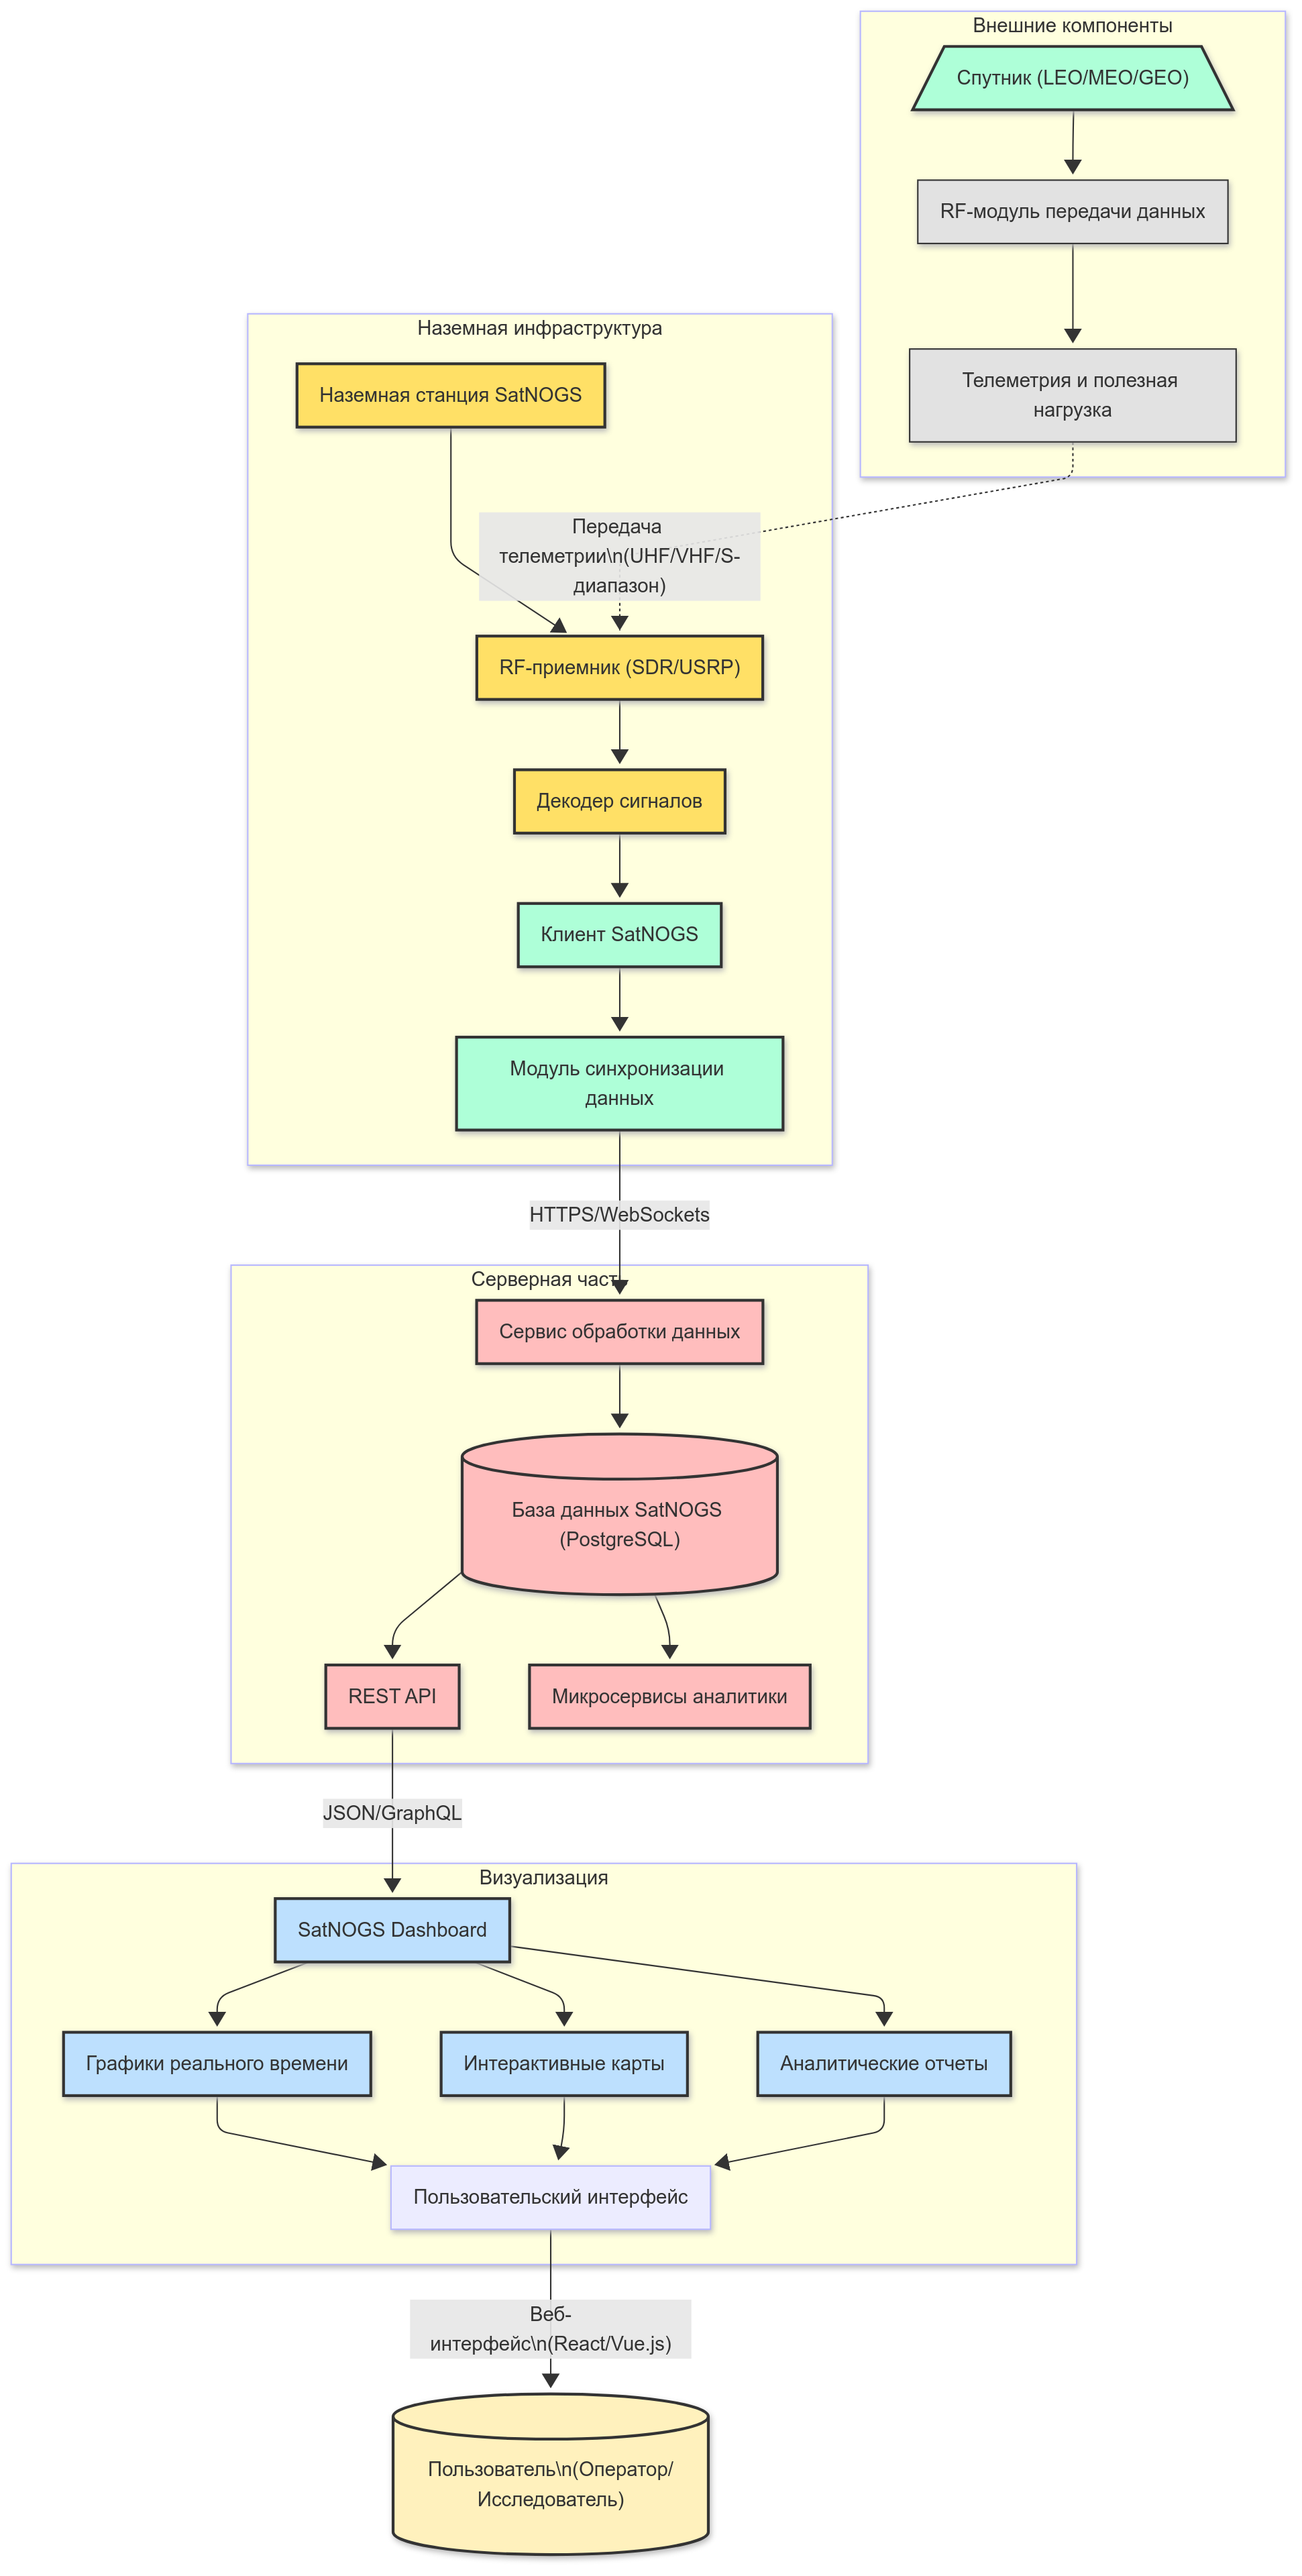
\includegraphics[width=0.4\textwidth]{satnogs_data_flow} \caption{Поток
		данных SatNOGS в Dashboard endpoint} \label{fig:satnogs_data_flow}
\end{figure}

\section{SatNOGS Dashboard}

\begin{figure}[htbp] \centering
	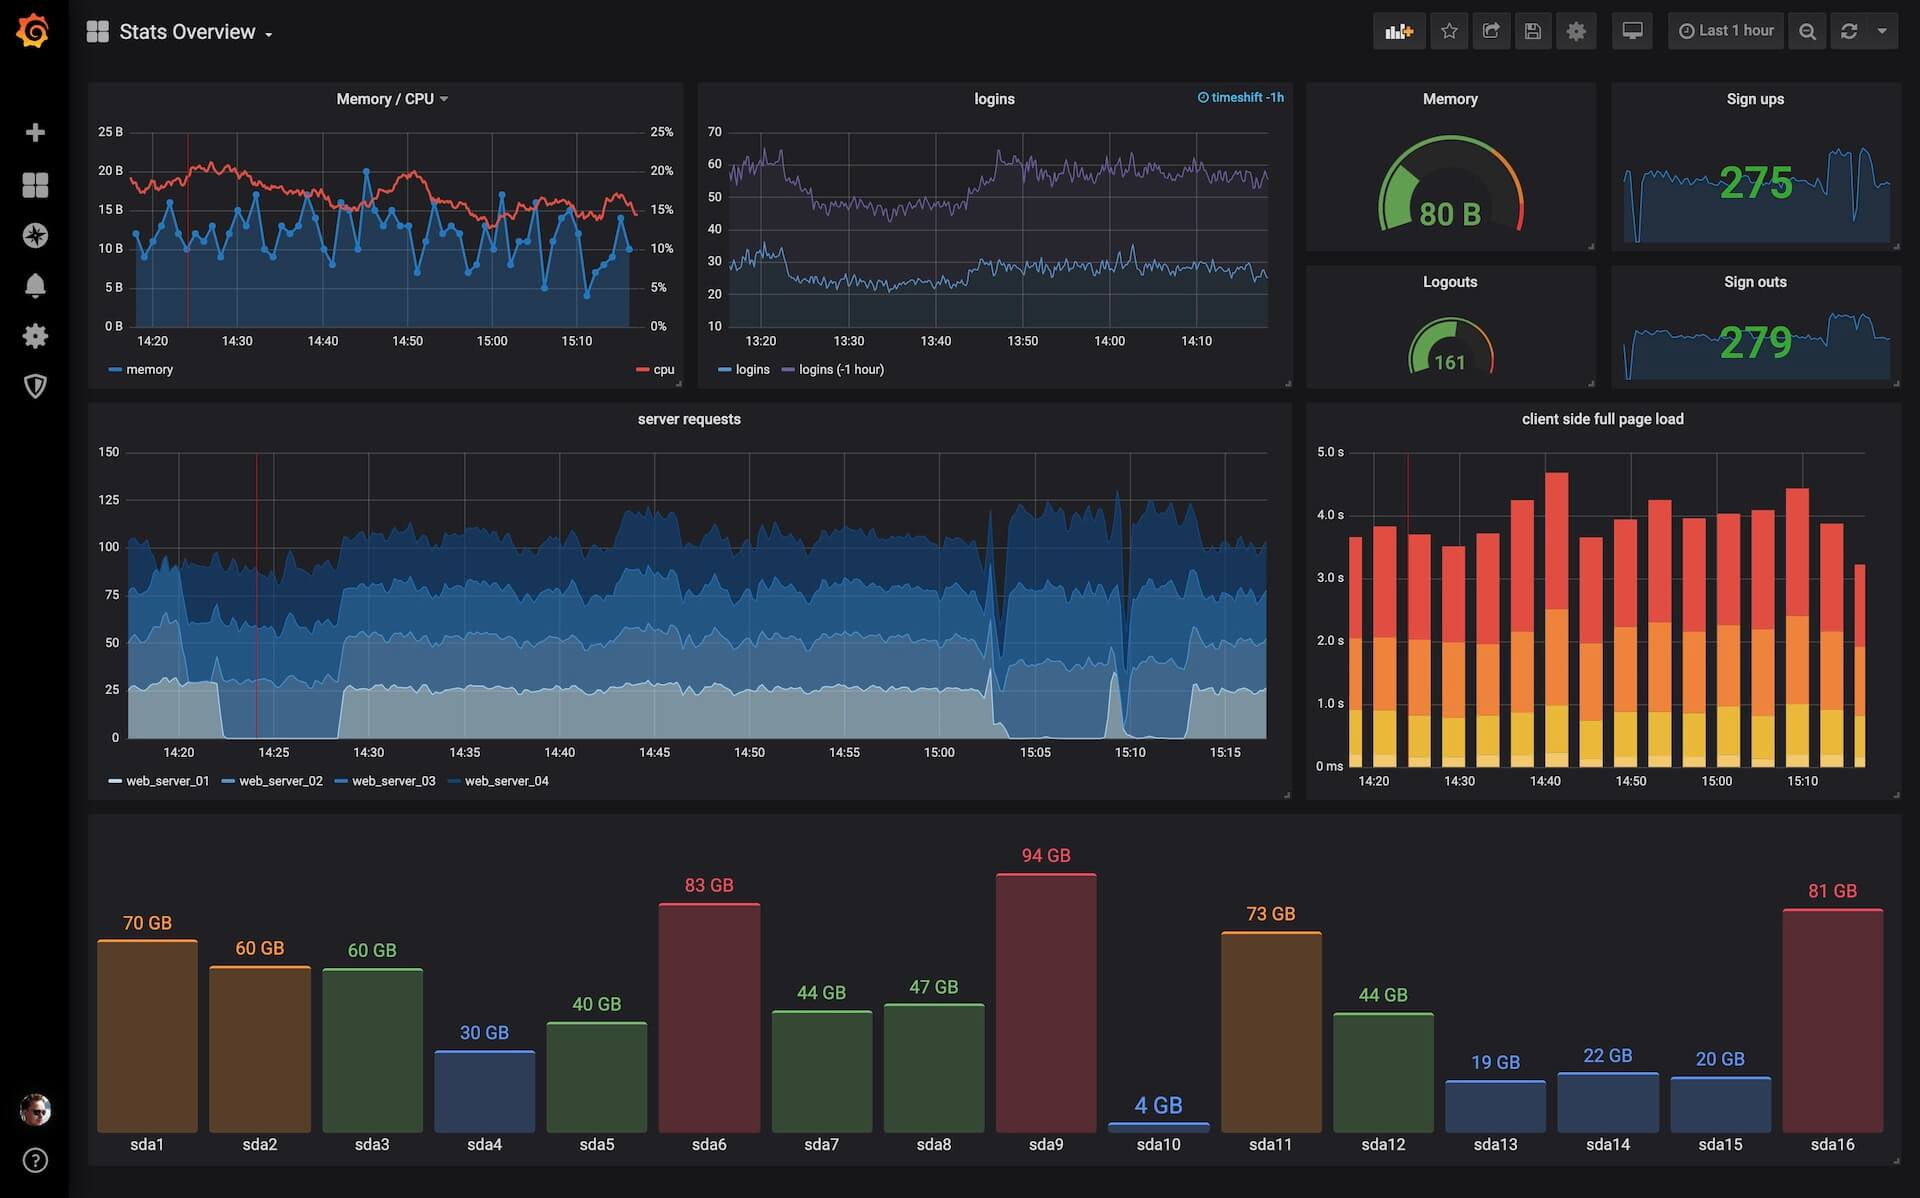
\includegraphics[width=1.0\textwidth]{grafana_example} \caption{Пример
		страницы с данными в Grafana Enterprise} \label{fig:grafana_example}
\end{figure}

Grafana — это мощная платформа для визуализации и анализа данных, которая
позволяет создавать интерактивные дашборды на основе различных источников
данных \cite{grafana_docs}. Пример такого дашборда можно увидеть на рисунке
\ref{fig:grafana_example}. Grafana широко используется для мониторинга систем
и приложений, предоставляя пользователям возможность отслеживать ключевые
метрики в реальном времени.

В контексте SatNOGS Dashboard, Grafana работает с базой данных
\textbf{InfluxDB} \cite{influxdb_docs}, которая предназначена для хранения
временных рядов данных, таких как телеметрия спутников. Данные поступают от
наземных станций, обрабатываются клиентом SatNOGS и сохраняются в InfluxDB.
Затем Grafana использует API для доступа к этим данным и их визуализации на
дашбордах.

Однако стоит отметить, что доступ к API Grafana Dashboard SatNOGS был закрыт,
что ограничивает возможности пользователей в получении данных напрямую. Более
того, Grafana не предоставляет свои услуги пользователям из России и Беларуси
\cite{grafana_community_post}, что создает дополнительные сложности для
разработчиков и исследователей из этих стран. Это делает Grafana ненадежной
платформой для работы в нашем регионе.

В связи с этими ограничениями нам приходится разрабатывать собственный парсер
для обхода существующих ограничений и получения необходимых данных. Этот
парсер будет рассмотрен далее в нашей работе, так как он позволит нам
интегрировать данные из SatNOGS Dashboard в нашу систему анализа и
визуализации.

Таким образом, несмотря на мощные возможности Grafana, текущие ограничения
доступа делают еe менее привлекательной для пользователей из определeнных
регионов, что требует разработки альтернативных решений для работы с данными.
Схему работы SatNOGS Dashboard можно наблюдать на рисунке
\ref{fig:grafana_infra}.

\begin{figure}[htbp] \centering
	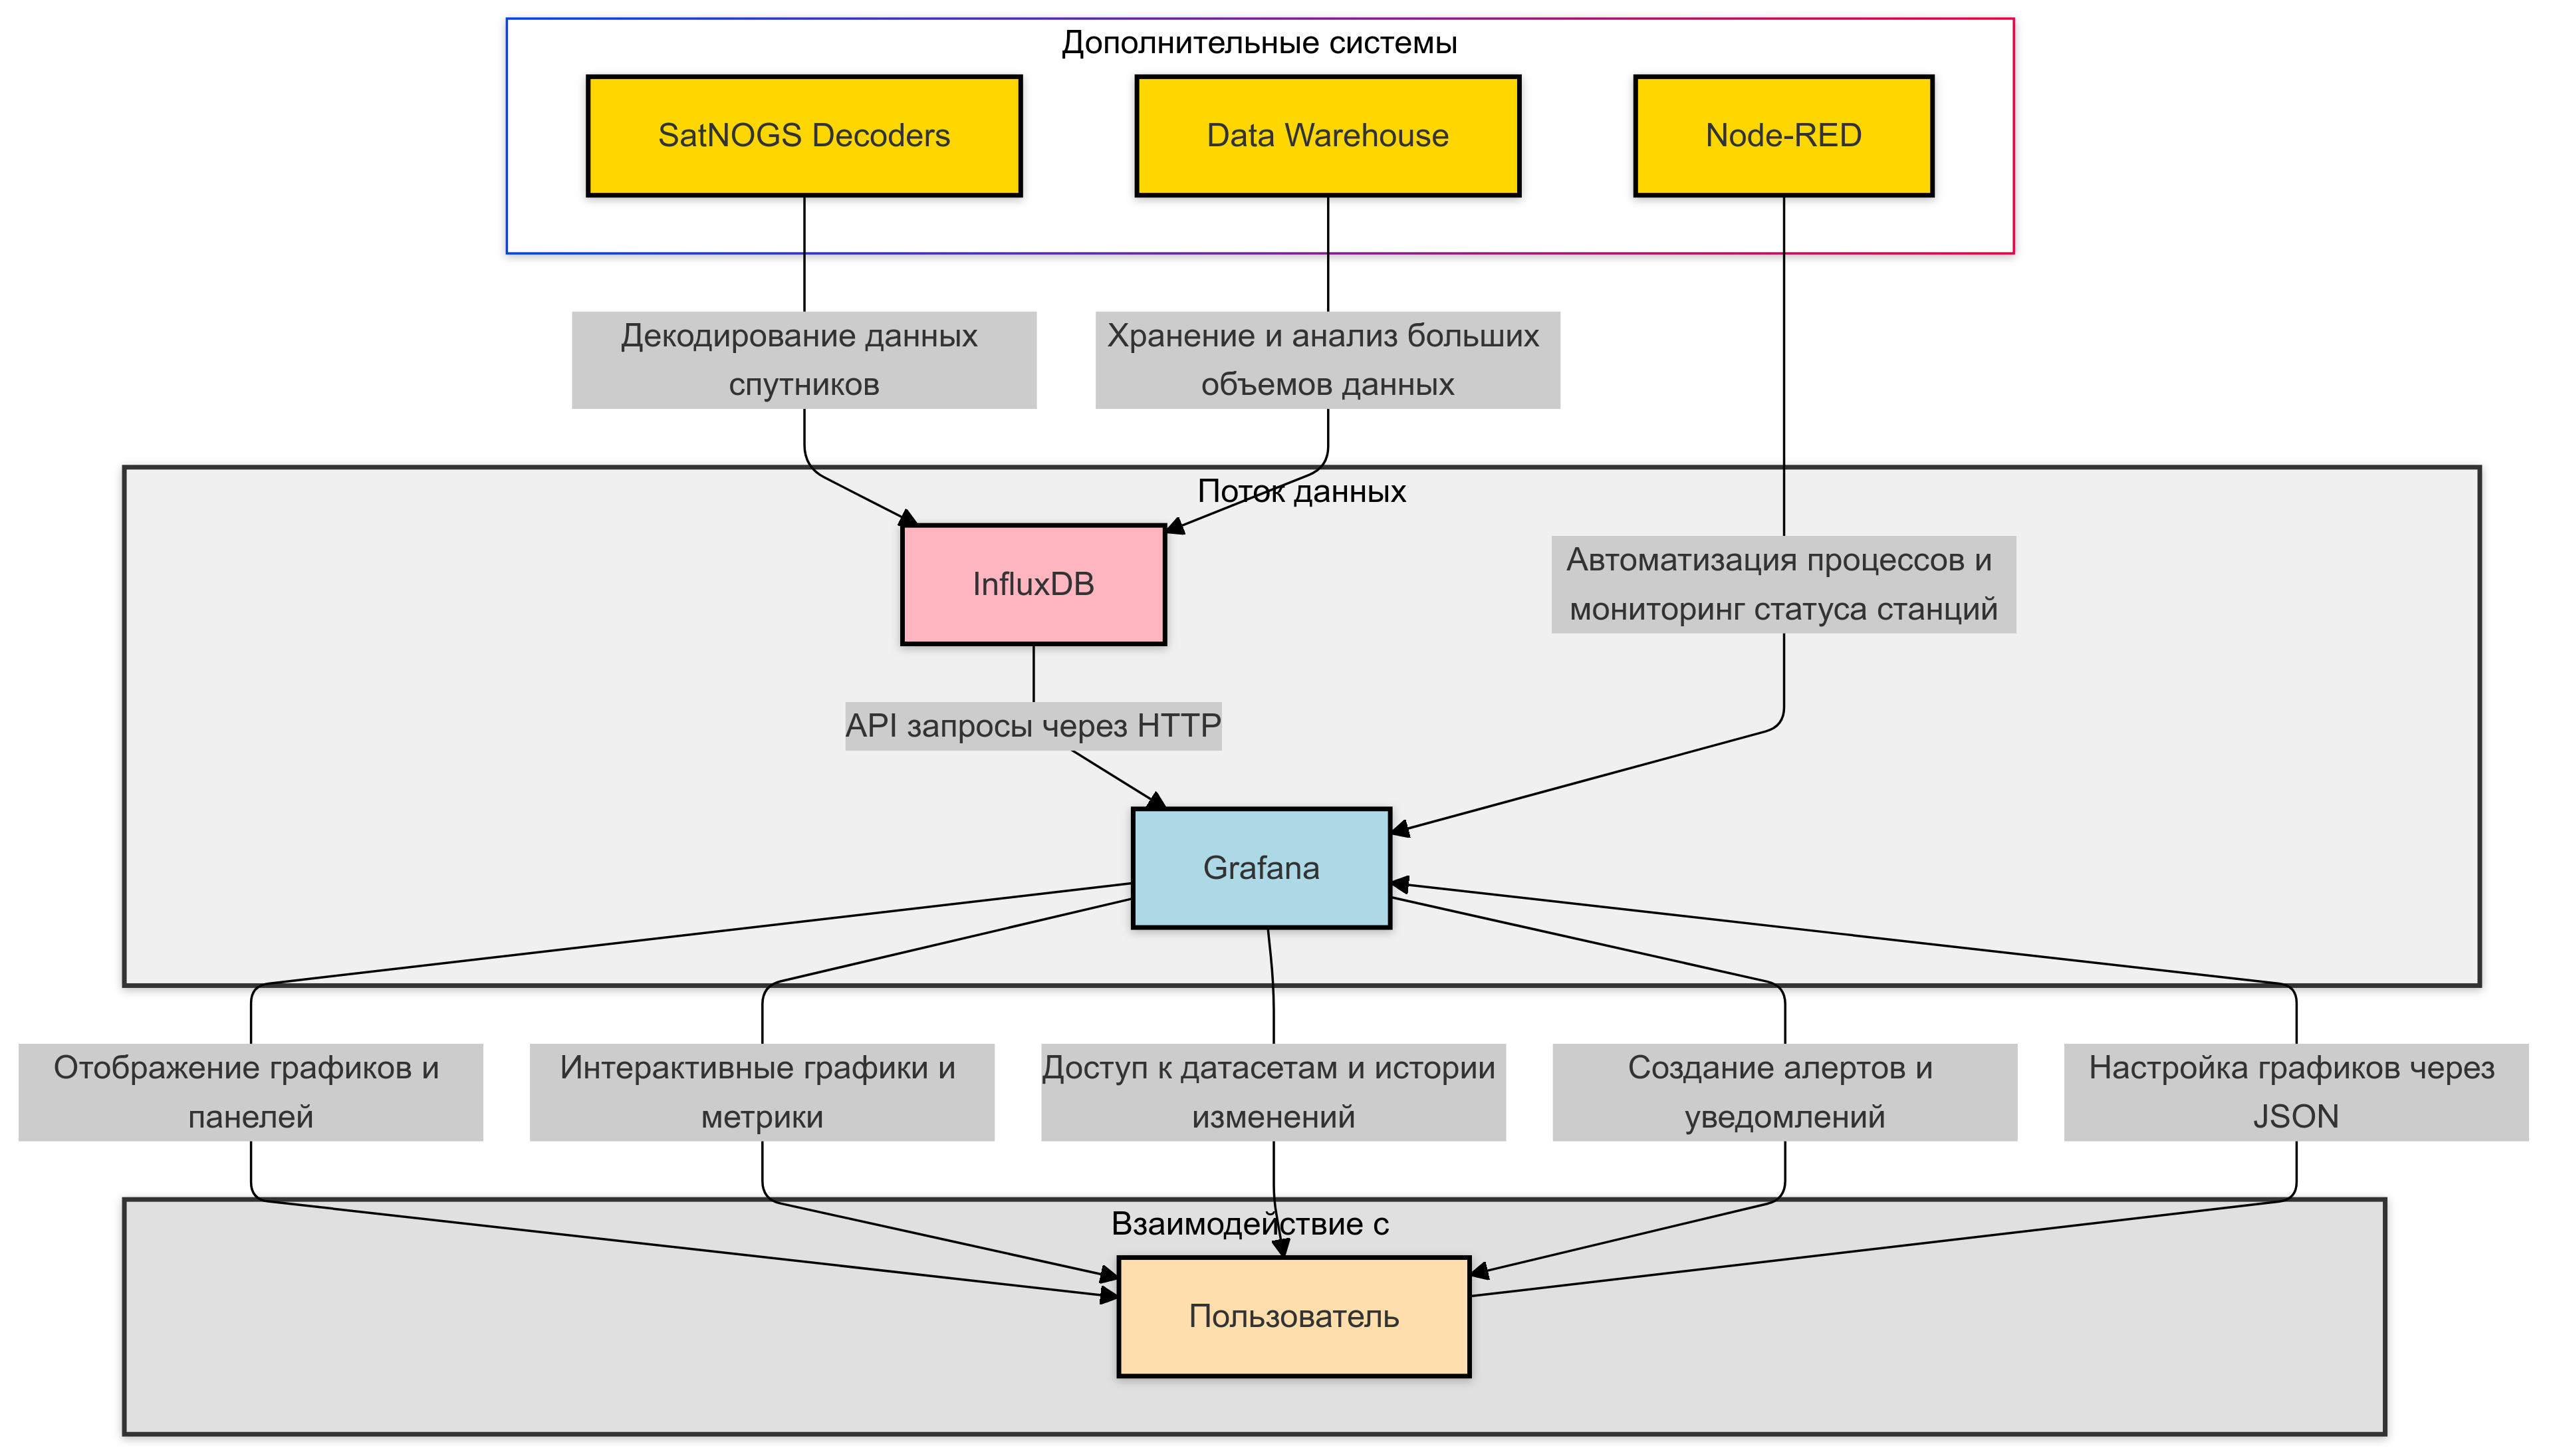
\includegraphics[width=1.0\textwidth]{grafana_infra} \caption{Подробное
		устройство SatNOGS Dashboard} \label{fig:grafana_infra} \end{figure}

\section{Парсинг SatNOGS Dashboard} \begin{figure}[htbp] \centering
	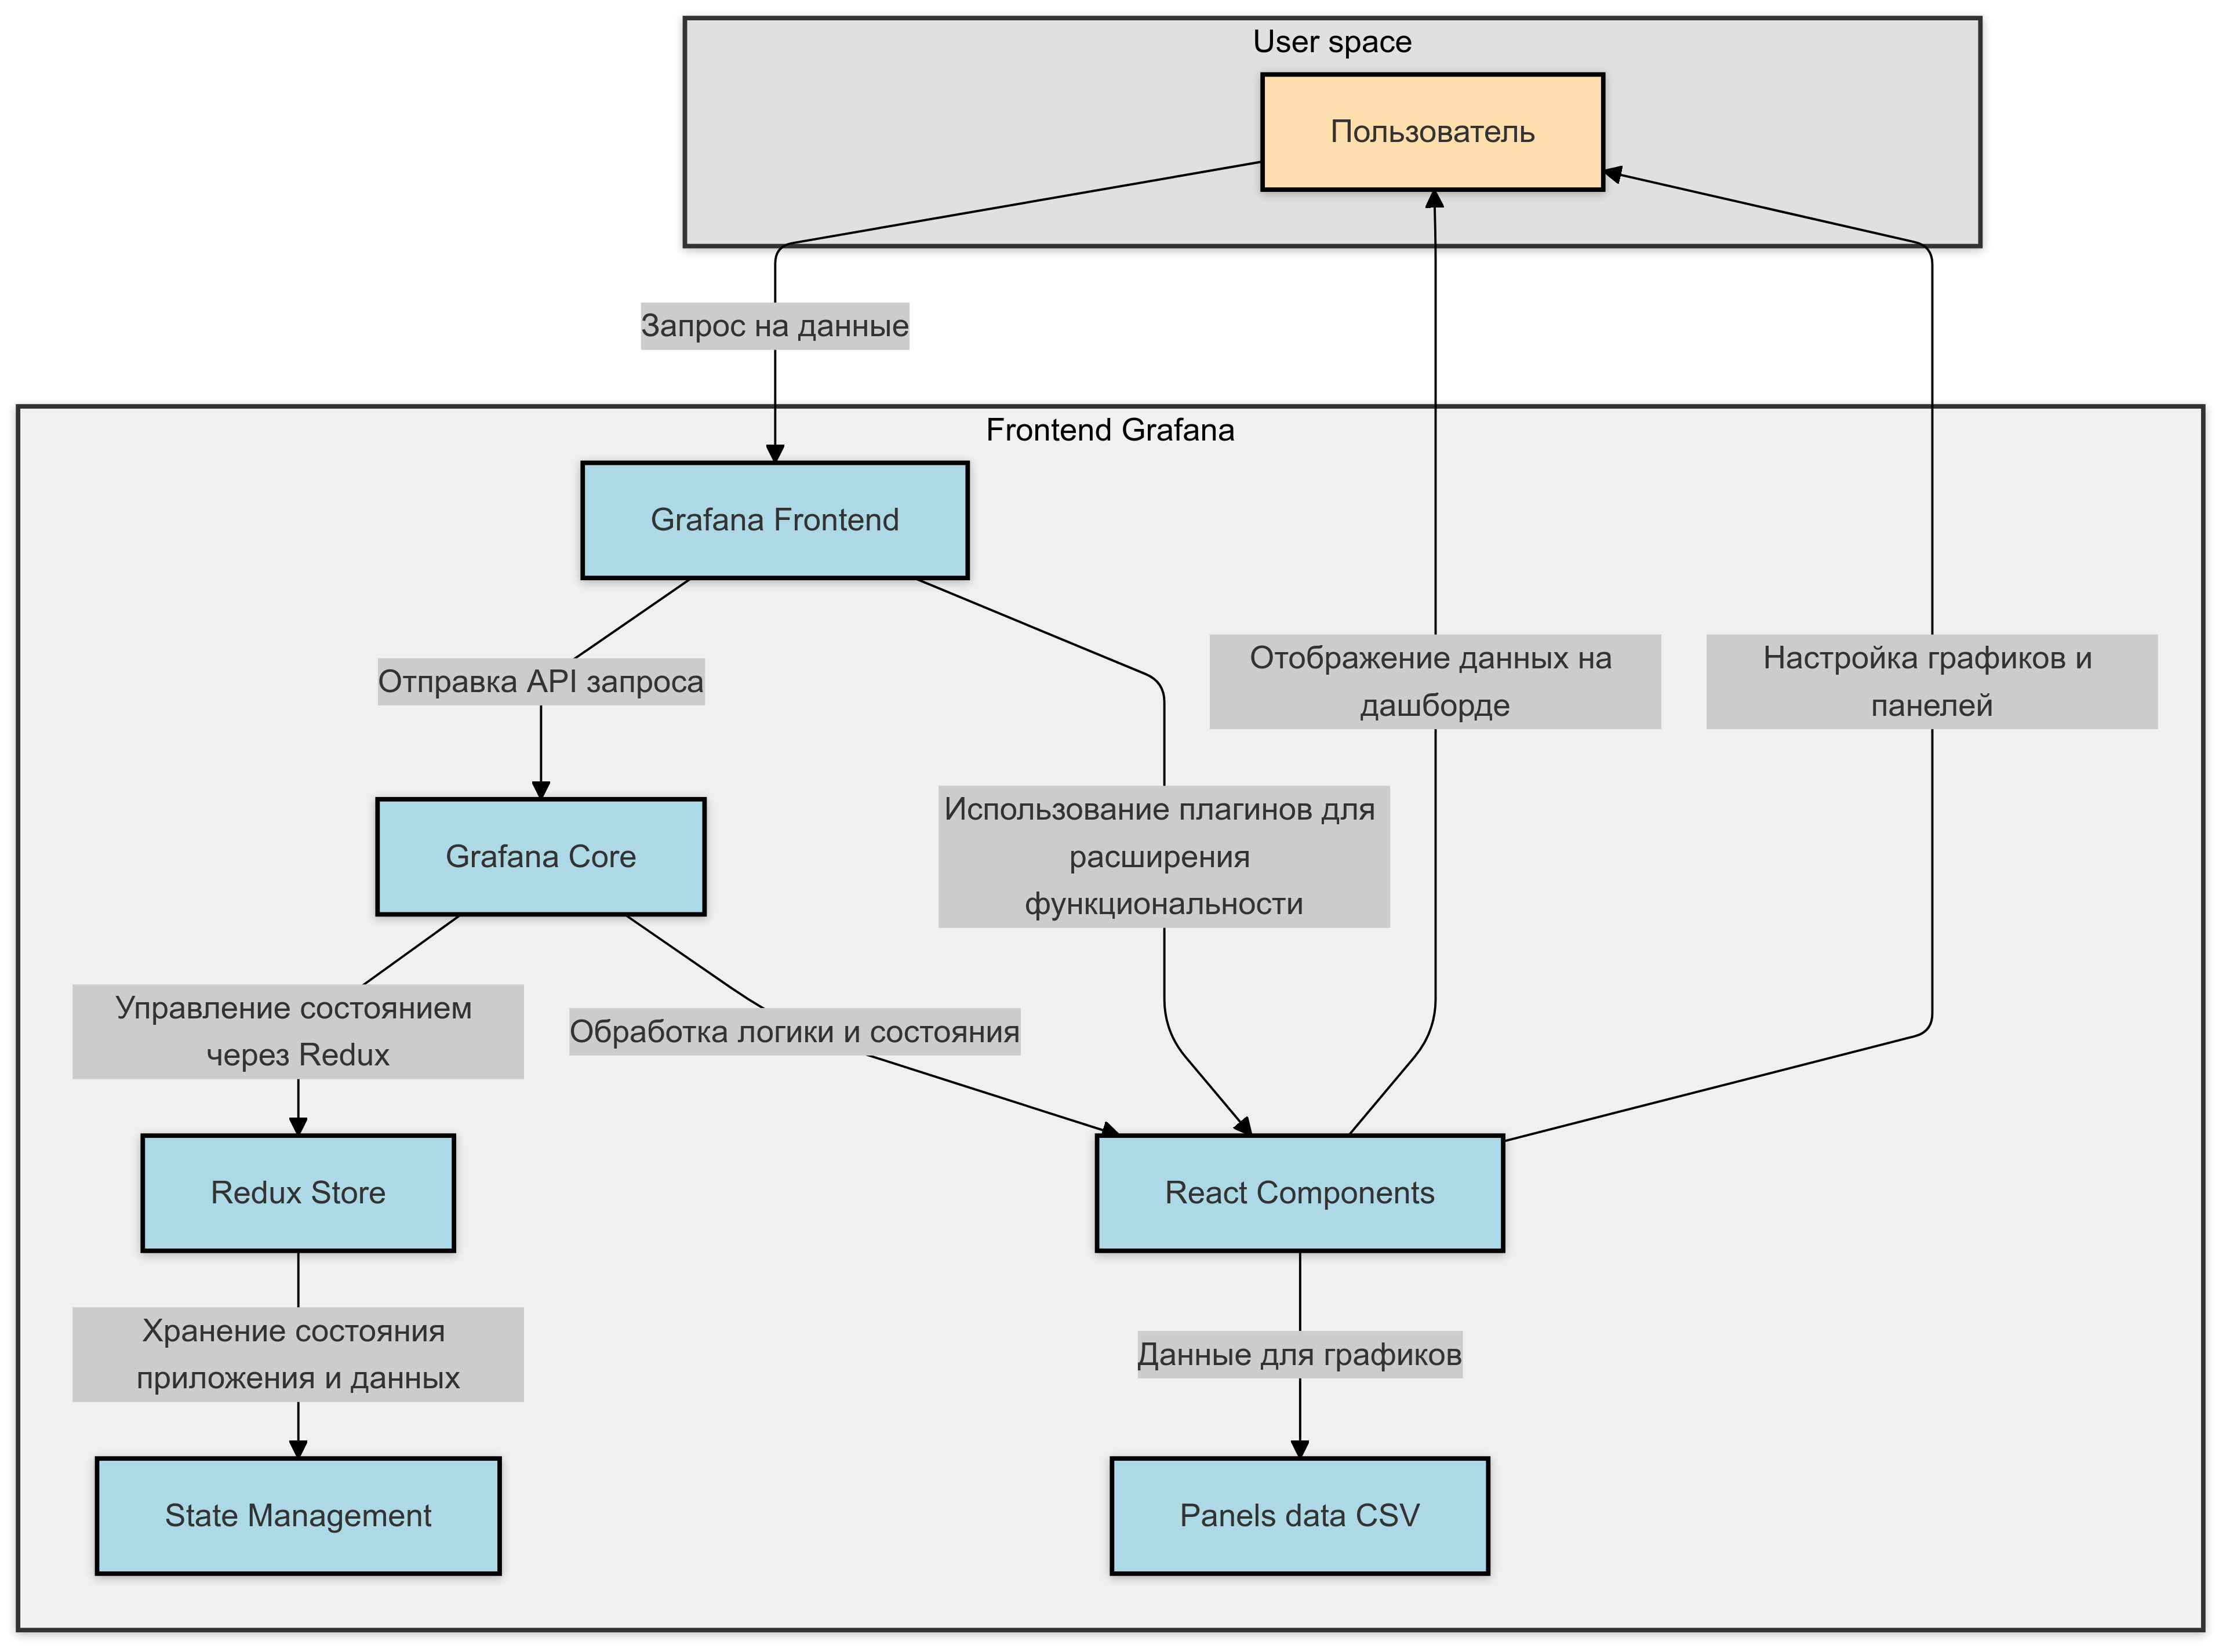
\includegraphics[width=1.0\textwidth]{grafana_frontend_structure}
	\caption{Построение frontend части grafana \cite{react_managing_state}}
	\label{fig:grafana_frontend_structure} \end{figure}

В рамках нашего проекта по анализу данных спутников мы столкнулись с
необходимостью работы с SatNOGS Dashboard. Это веб-интерфейс, который
предоставляет доступ к данным о спутниках и их телеметрии. Однако,
поскольку API для этого интерфейса является приватным, мы вынуждены
прибегать к парсингу фронтенда с использованием JavaScript, см. рисунок
\ref{fig:grafana_frontend_structure}.

Для начала, мы используем JavaScript для извлечения необходимых данных из
DOM-структуры страницы. Это позволяет нам взаимодействовать с элементами
интерфейса и получать информацию, которая в противном случае была бы
недоступна. Мы реализуем асинхронные функции для ожидания появления
элементов на странице и их обработки.

После того как данные извлечены с помощью JavaScript, мы запускаем скрипт
на Python с использованием библиотеки Selenium WebDriver
\cite{selenium_docs}. Этот подход позволяет автоматизировать взаимодействие
с веб-интерфейсом SatNOGS в нужный момент времени.

Что касается инфраструктуры, мы используем Grafana для визуализации данных.
Grafana интегрируется с различными источниками данных и позволяет создавать
настраиваемые дашборды для мониторинга состояния спутников и анализа
телеметрии. API Grafana предоставляет возможности для динамического
обновления графиков и управления панелями.

Таким образом, мы не только извлекаем данные из SatNOGS Dashboard, но и
используем мощную инфраструктуру для их анализа и визуализации.

\section{Работа скрипта для загрузки данных из Grafana}

Скрипт, написанный на Python с использованием библиотеки Selenium,
предназначен для автоматизации процесса извлечения данных из дашборда
Grafana. Он начинается с настройки логирования и создания веб-драйвера для
браузера Firefox с необходимыми параметрами, такими как директория для
загрузки файлов и типы файлов, которые могут загружаться без подтверждения.

После инициализации драйвера скрипт переходит к идентификации панелей на
дашборде. Он перебирает идентификаторы панелей и проверяет наличие
элементов с соответствующими идентификаторами. Если элемент найден, его
заголовок добавляется в список доступных панелей.

Далее скрипт формирует полный URL для доступа к дашборду с учетом временных
параметров. После загрузки страницы он получает список панелей и создает
новый URL для каждой панели с параметром инспекции. Скрипт ожидает
появления необходимых элементов на странице и инициирует процесс загрузки
данных через выполнение вышеописанного JavaScript-кода.

В заключение, основной блок скрипта определяет список URL-адресов
дашбордов, откуда необходимо загружать данные, и создает директорию для
сохранения загружаемых файлов. В результате работы данного скрипта
происходит автоматическая загрузка данных из Grafana, что значительно
упрощает процесс извлечения информации для дальнейшего анализа или
хранения.


\newpage

\chapter{Глубокая модификация Polaris ML: polaris 2.0}

\section{Исходная модель}

Polaris ML — это платформа машинного обучения, разработанная LibreSpace
Foundation ~\cite{librespace_docs} для анализа данных телеметрии спутников.
Основная цель платформы заключается в автоматизации анализа данных телеметрии,
что позволяет своевременно выявлять аномалии, визуализировать временные ряды
параметров бортовых систем и строить прогнозные модели на основе исторических
данных ~\cite{ray_2002_bayesian}. Эти функции делают Polaris ML важным
инструментом в мониторинге состояния спутников и обеспечении их стабильной
работы \cite{polaris_ml_docs}.

Техническая реализация LSF Polaris ML основывается на использовании упрощенного
алгоритма XGBoost. Этот алгоритм был выбран благодаря своей эффективности при
работе с малым количеством данных и высокой интерпретируемости результатов.

Алгоритм XGBoost играет ключевую роль в работе Polaris ML. Его высокая скорость
обучения и встроенная поддержка обработки пропущенных данных обеспечивают
надежность анализа. Кроме того, благодаря возможностям XGBoost интерпретировать
влияние отдельных признаков на результат, платформу можно использовать для
детального изучения взаимосвязей между параметрами бортовых систем спутника
\cite{xgboost_docs}. Таким образом, Polaris ML представляет собой мощный
инструмент для управления и анализа спутниковых данных, обеспечивая более
глубокое понимание процессов, происходящих на борту.

\section{Проблемы исходной модели и их решение}

Однако, как было отмечено ранее, в платформе Polaris ML используется
стандартный, упрощенный вариант XGBoost, который ограничивается малым
количеством оптимизируемых гиперпараметров. Такой подход позволяет упростить
процесс настройки модели и сохранить вычислительную эффективность, что особенно
важно в контексте обработки больших потоков телеметрических данных в реальном
времени. Тем не менее, данный метод имеет свои ограничения.

Алгоритм XGBoost в Polaris ML конфигурируется через сеточный поиск
гиперпараметров (grid search), который является одной из самых простых, но
далеко не самых эффективных стратегий оптимизации. Сеточный поиск представляет
собой перебор фиксированного набора параметров по заранее определенной сетке,
что может быть вычислительно затратным, особенно при увеличении размерности
гиперпараметров. Кроме того, он не учитывает возможные взаимодействия между
параметрами и не адаптируется в зависимости от текущих результатов оптимизации.
Это может привести к пропуску оптимальных значений параметров или необходимости
значительного увеличения вычислительных ресурсов для достижения
удовлетворительных результатов.

В последние годы появились более совершенные методы оптимизации гиперпараметров
\cite{grid_search_tuning}, такие как Halving Grid Search, Random Search и
Bayesian Optimization. Halving Grid Search, например, использует итеративное
уменьшение пространства поиска, концентрируясь на наиболее перспективных
комбинациях параметров. Это позволяет существенно сократить время подбора,
особенно при использовании перекрестной валидации (cross-validation), которая
увеличивает точность оценки моделей, но также повышает вычислительную нагрузку.

С другой стороны, Random Search предоставляет гибкость за счет случайного
выбора комбинаций параметров в заданных диапазонах \cite{grid_search_tuning}.
Исследования показывают, что этот подход может находить оптимальные параметры
быстрее, чем сеточный поиск, особенно в задачах с высокой размерностью
пространства параметров. Bayesian Optimization \cite{grid_search_tuning},
напротив, активно использует предыдущие результаты для предсказания наиболее
вероятных успешных параметров, обеспечивая баланс между исследованием нового
пространства и уточнением уже исследованного.

В данный момент в рамках платформы Polaris ML реализуются значительные
изменения, направленные на повышение производительности, удобства использования
и расширение функционала. Одним из ключевых направлений стало перенесение
инфраструктуры с Python на C++. Это изменение продиктовано необходимостью
оптимизации вычислений и улучшения управления памятью, что особенно актуально
при обработке больших объемов данных телеметрии. Такой перенос позволяет
эффективно использовать ресурсы оборудования и минимизировать задержки,
возникающие при работе с динамически типизированными языками.

В рамках этих работ также внедряется распределение нагрузки по ядрам процессора
для создания деревьев и обучения малых моделей. Такой подход позволяет
максимально задействовать возможности многоядерных систем и сократить время
обработки данных, особенно при выполнении параллельных вычислений.

\section{Новый формат входных данных}

Существенные изменения коснулись и самих данных \ref{fig:polaris_data_flow}.
Теперь используется увеличенный объем входных данных, что способствует созданию
более точных и устойчивых моделей. В дополнение к этому появилась возможность
добавлять собственные данные о солнечной активности, оформленные в формате
pandas DataFrame. Ранее такая возможность была доступна только для спутниковых
данных, и пользователям приходилось самостоятельно декодировать их перед
использованием. Устранение этапа декодирования кадров стало важным шагом
вперед: теперь данные загружаются напрямую из SatNOGS Grafana Dashboard, что
существенно упрощает их обработку. Прямое формирование DataFrame избавляет
пользователей от необходимости выполнения промежуточных операций, таких как
обработка сетевых потоков или декодирование.

\begin{figure}[htbp] \centering
	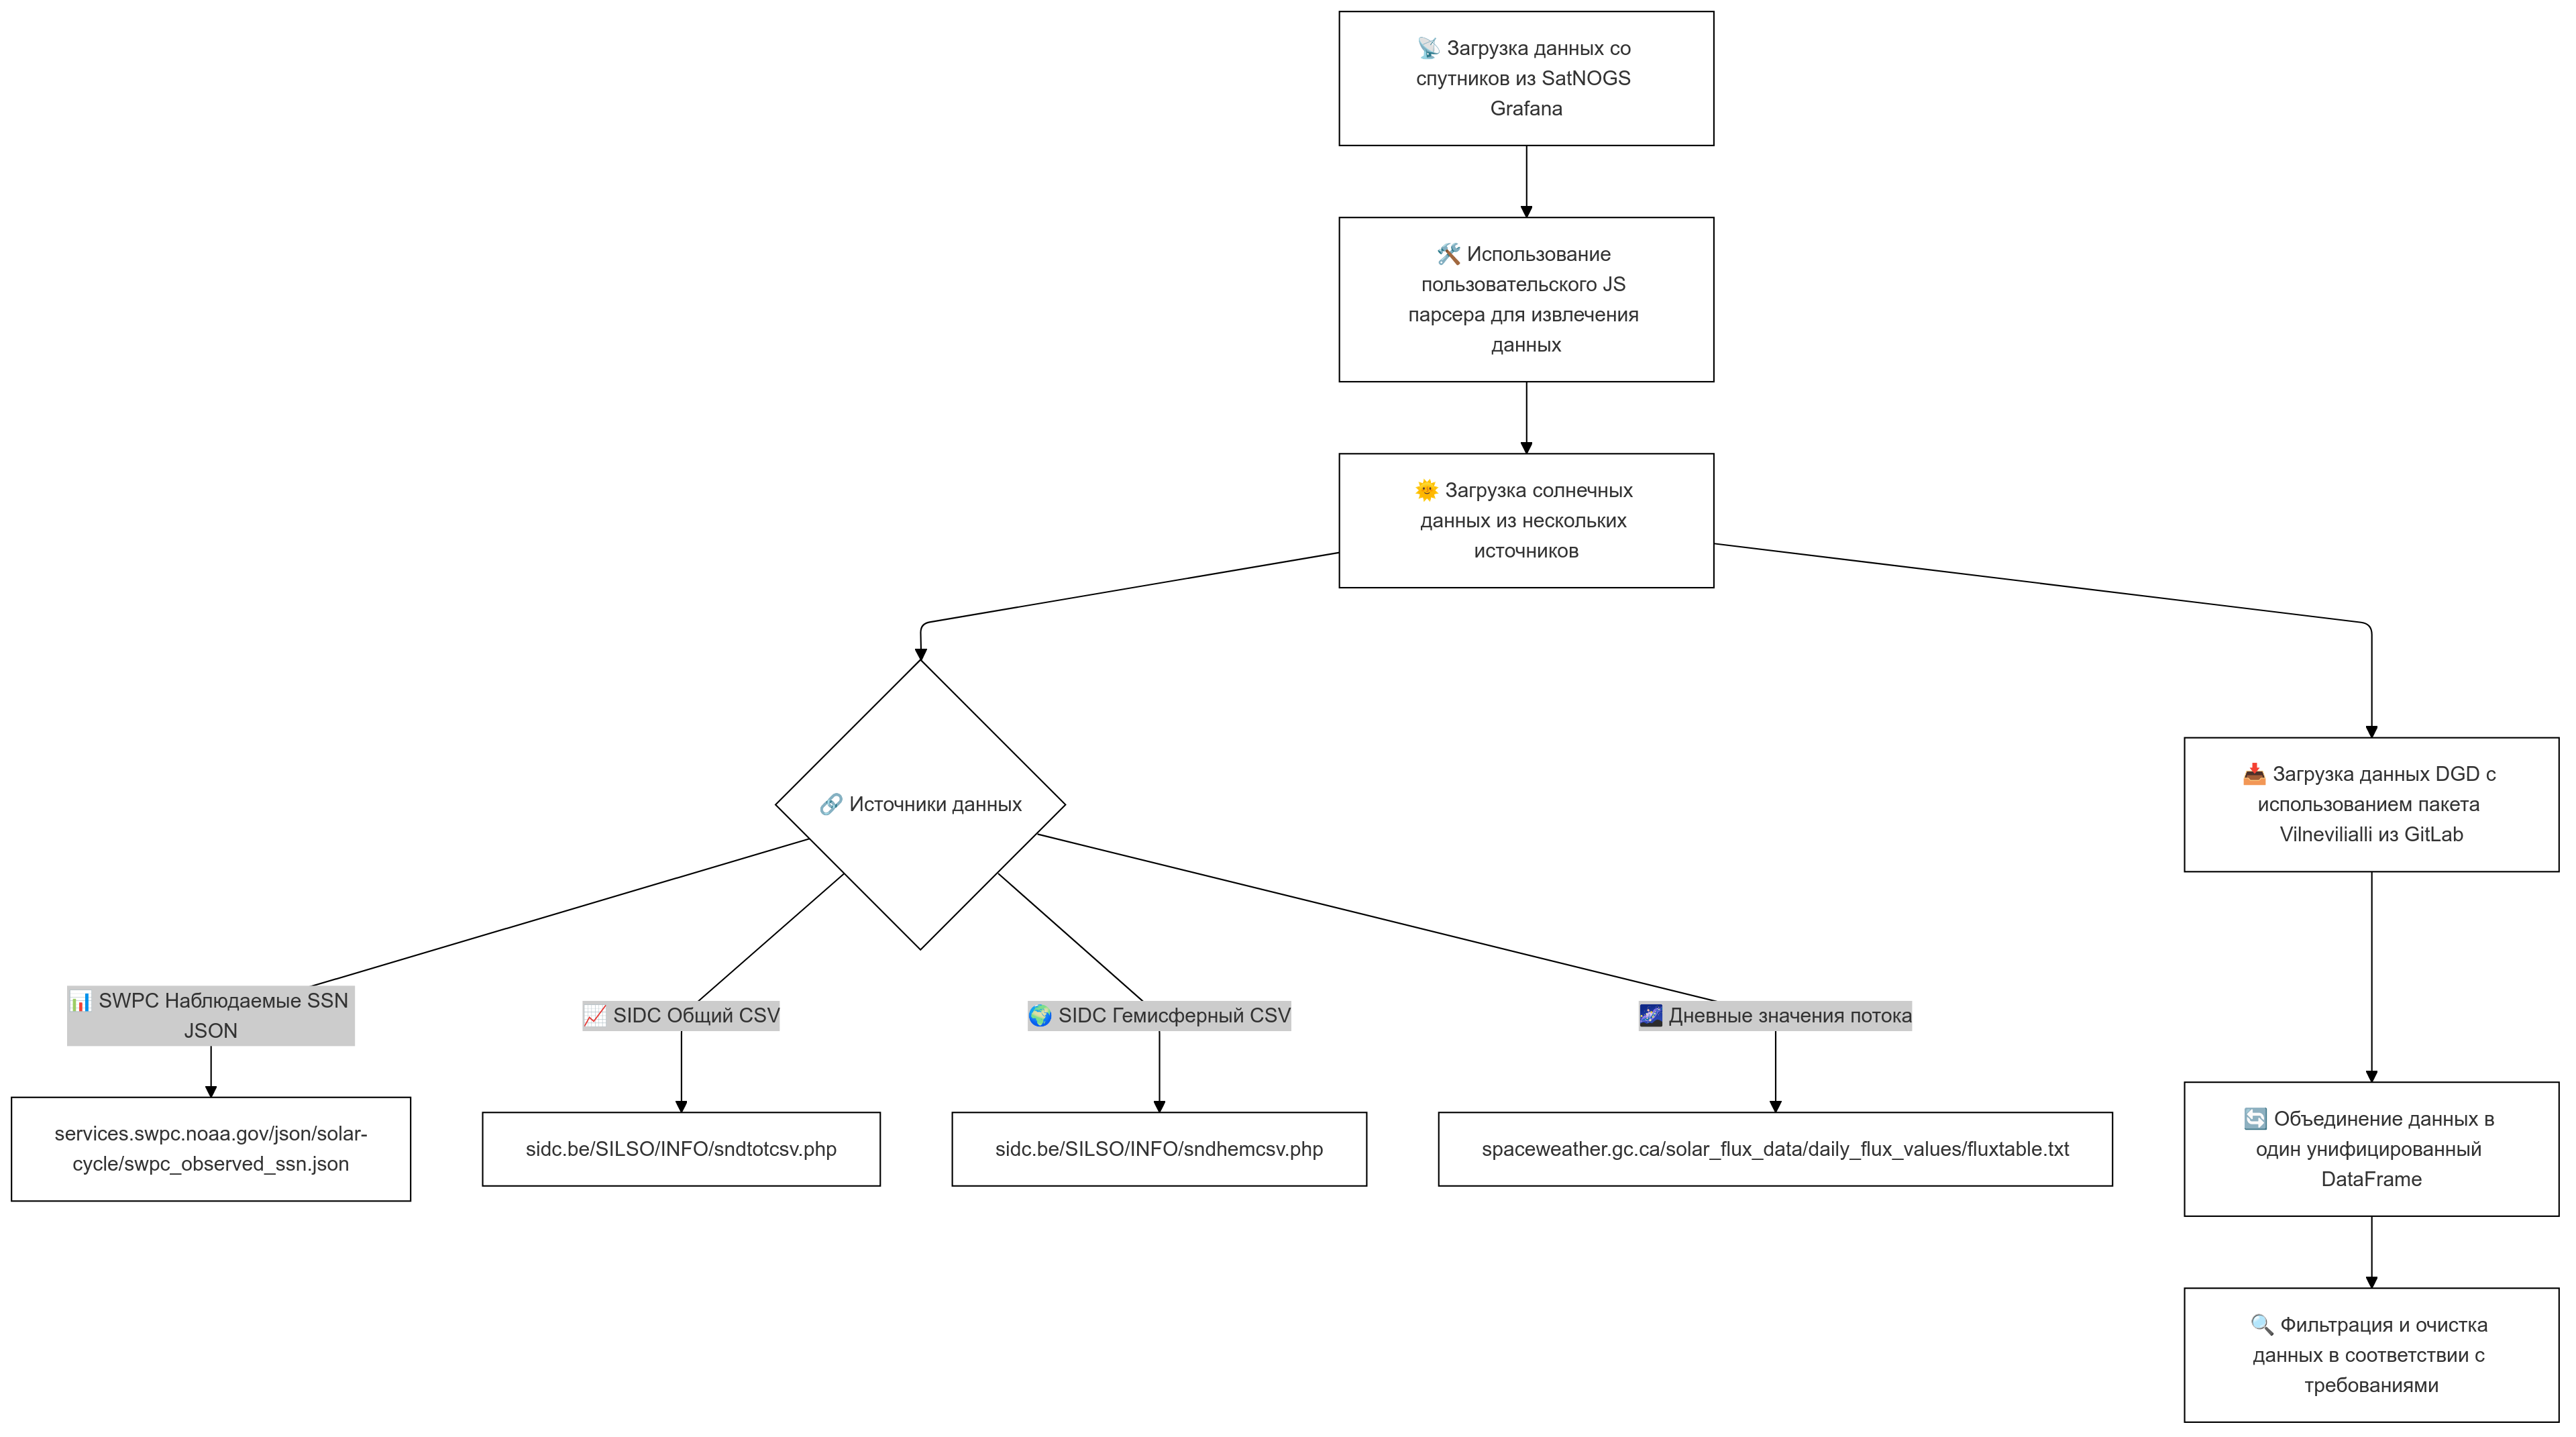
\includegraphics[width=1.0\textwidth]{polaris_data_flow} \caption{Измененный
		входной поток данных для polaris 2.0} \label{fig:polaris_data_flow}
\end{figure}

\section{Новый формат графа связности}

Для визуализации данных и анализа их взаимосвязей было принято решение о
переносе построения графов на внешнюю библиотеку pyecharts
\cite{pyecharts_docs}. Это изменение не только устранило необходимость
взаимодействия с Node.js-проектами, но и значительно упростило создание
графиков и визуализаций, которые теперь могут быть интегрированы в отчетность и
презентации без лишних трудозатрат. Кроме того, интеграция с библиотекой
pyecharts обеспечила гибкость в настройке визуализаций и расширила возможности
по взаимодействию с интерактивными элементами.

Для управления процессами обучения и экспериментов внедрен mlflow
\cite{mlflow_docs}, который позволил стандартизировать ведение отчетности.
Теперь в отчетный журнал можно автоматически сохранять артефакты обучения,
такие как модели, параметры, метрики и визуализации. Это упрощает анализ и
повторное использование ранее выполненных экспериментов. Локально развернутый
MLflow UI-сервер позволяет интерактивно сравнивать различные модели с
различными гиперпараметрами. Это делает процесс подбора параметров прозрачным и
управляемым, особенно при использовании новых возможностей для оптимизации до
30 параметров XGBoost.

В числе таких параметров — $gamma$, $max\_depth$, $min\_child\_weight$,
$subsample$ и многие другие. Расширенный набор конфигураций позволяет детально
подстраивать поведение модели под конкретные задачи. Переход к работе с
увеличенным количеством гиперпараметров сделал платформу более гибкой, а
процессы обучения — более детализированными.

Еще одним важным улучшением стало перенесение данных в память GPU с оптимальной
упаковкой для ускоренного доступа. Это изменение дало значительный прирост в
скорости обучения моделей за счет устранения узких мест, связанных с задержками
при чтении и записи данных в оперативной памяти. Теперь платформе доступны
преимущества параллельных вычислений, которые обеспечивают современные
графические процессоры.

В целом, сделан упор на удобство MLOps и упрощение конфигурирования сети
\ref{fig:polaris_core}. Это включает в себя автоматизацию ряда рутинных
процессов, связанных с подготовкой данных, настройкой экспериментов и ведением
отчетности. Эти изменения обеспечивают не только повышение производительности,
но и улучшение пользовательского опыта для инженеров, работающих с Polaris ML.
Платформа становится не просто инструментом для анализа телеметрии, но и
полноценной экосистемой для управления данными, экспериментами и визуализацией
результатов.

\begin{figure}[htbp] \centering
	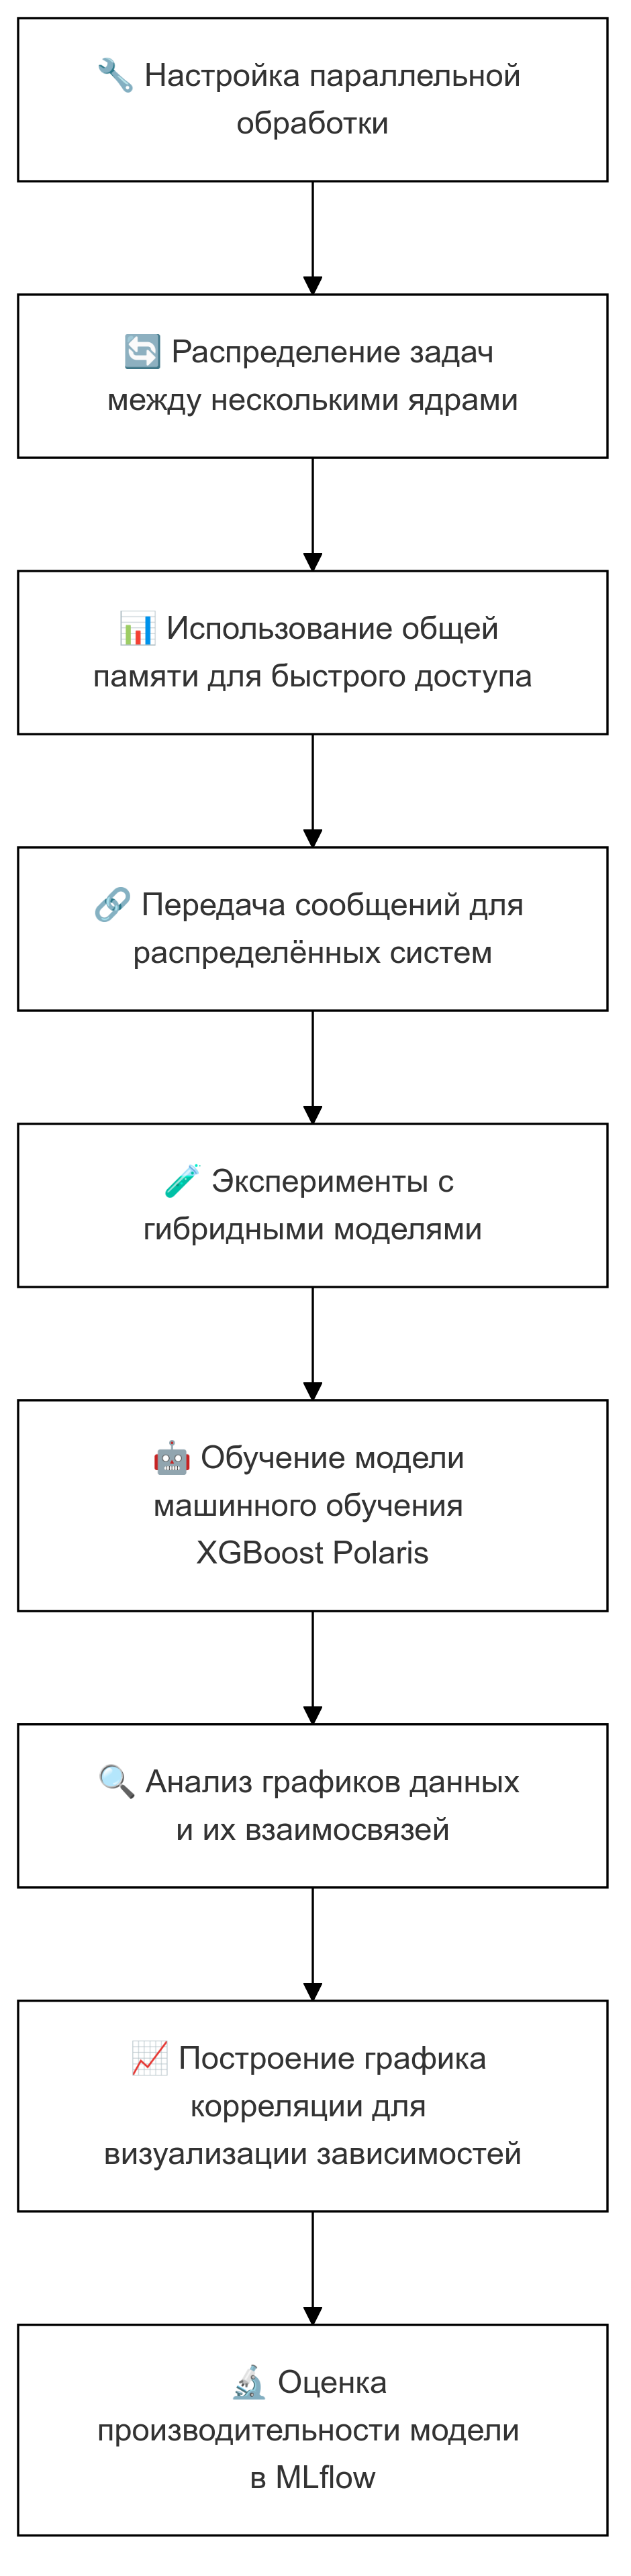
\includegraphics[width=0.34\textwidth]{polaris_core} \caption{Ядро polaris 2.0}
	\label{fig:polaris_core} \end{figure}

В данной таблице представлены основные конфигурируемые и grid-оптимизируемые
параметры модели XGBoost \cite{xgboost_parameters_docs}, их описание и значения
по умолчанию. Параметры разделены на три категории: общие параметры, параметры
бустера и параметры задачи.

\begin{longtable}{|p{4cm}|p{6cm}|p{6cm}|} \caption{Параметры XGBoost и их
		влияние}\label{tab:xgboost_params}
	\\

	\hline \textbf{Параметр}                          & \textbf{Описание}
	                                                  & \textbf{Влияние}
	\\ \hline \endfirsthead

	\multicolumn{3}{c} {\tablename\ \thetable\ -- \textit{Продолжение}}
	\\ \hline \textbf{Параметр}             & \textbf{Описание}
	                                                  & \textbf{Влияние}
	\\ \hline \endhead

	\hline \multicolumn{3}{|r|}{\textit{Продолжение на следующей странице}}
	\\ \hline \endfoot

	\hline \endlastfoot

	\texttt{eta (learning\_rate)}                     & Скорость обучения, регулирует вес новых
	деревьев                                          & Слишком низкое значение может привести к недообучению,
	слишком высокое — к переобучению                                                                                                \\ \hline \texttt{gamma}                &
	Минимальный прирост в качестве для разбиения узла & Увеличение
	значения приводит к более простой модели
	\\ \hline \texttt{max\_depth}           & Максимальная глубина деревьев
	                                                  & Большее значение увеличивает мощность модели, но повышает риск переобучения
	\\ \hline \texttt{subsample}            & Доля данных, используемая для
	обучения каждого дерева                           & Снижает переобучение, но может ухудшить
	точность модели                                                                                                                 \\ \hline
	\texttt{colsample\_bytree}                        & Доля признаков, используемых для обучения
	каждого дерева                                    & Уменьшение значения предотвращает переобучение
	\\ \hline \texttt{lambda (reg\_lambda)} & L2-регуляризация на веса
	                                                  & Увеличение значения уменьшает переобучение
	\\ \hline \texttt{alpha (reg\_alpha)}   & L1-регуляризация на веса
	                                                  & Способствует разреженности модели и снижает переобучение
	\\ \hline \texttt{scale\_pos\_weight}   & Вес положительных примеров для
	несбалансированных классов                        & Полезно для работы с несбалансированными данными
	\\ \hline \texttt{min\_child\_weight}   & Минимальная сумма весов наблюдений
	в узле                                            & Увеличение значения приводит к более простой модели
	\\ \hline \texttt{n\_estimators}        & Количество деревьев в ансамбле
	                                                  & Большее количество может улучшить точность, но увеличивает время обучения
	\\\end{longtable}


\chapter{MLflow: История Экспериментов в Зависимости от Параметров}

В последние годы платформы для управления экспериментами, такие как MLflow,
играют важную роль в эффективной организации процессов машинного обучения. В
контексте Polaris ML MLflow стал неотъемлемым инструментом для отслеживания,
управления и повторного использования экспериментальных данных. Благодаря
интеграции с MLflow, инженерный процесс стал значительно более прозрачным, а
результаты экспериментов — более доступными для анализа и визуализации.

\section{Основные Возможности MLflow}

MLflow предоставляет целый ряд возможностей, которые позволяют эффективно
управлять жизненным циклом моделей машинного обучения \cite{mlflow_docs}:

\begin{itemize} \item \textbf{Отслеживание экспериментов.} MLflow позволяет
	      вести журнал экспериментов с возможностью фиксировать параметры, метрики,
	      артефакты и модели. Все эти данные автоматически сохраняются в базе
	      данных или локальном сервере. \item \textbf{Сравнение моделей.} MLflow
	      предлагает удобный интерфейс для сравнения различных экспериментов и
	      моделей, что упрощает процесс подбора гиперпараметров. \item
	      \textbf{Артефакты.} После завершения эксперимента в MLflow
	      сохраняются артефакты, такие как визуализации, модели и файлы, что
	      позволяет легко делиться результатами и восстанавливать предыдущие
	      эксперименты. \item \textbf{Интерактивный интерфейс.} MLflow UI
	      предоставляет пользователям удобный веб-интерфейс для
	      взаимодействия с результатами экспериментов, что упрощает анализ и
	      визуализацию метрик и артефактов. \end{itemize}

\section{Интеграция MLflow в Polaris ML}

Интеграция MLflow в платформу Polaris ML позволила значительно
улучшить управление экспериментами и создание отчетности. Теперь
каждый эксперимент фиксируется в системе с метками параметров,
гиперпараметров, метрик и полученных результатов, что обеспечивает
гибкость в анализе и повторении экспериментов. В рамках Polaris ML
используется локальный сервер MLflow, который позволяет работать с
экспериментами без необходимости подключения к удаленным сервисам,
ускоряя процесс разработки и оптимизации.

\section{Артефакты MLflow}

После каждого эксперимента, помимо метрик, сохраняются
разнообразные артефакты, которые помогают наглядно оценить
результаты работы модели. Эти артефакты включают важные элементы,
такие как важность признаков, остатки предсказаний, распределения
ошибок и другие визуализации.

\subsection{Важность Признаков}

Важность признаков — ключевая метрика для оценки значимости
различных переменных в модели. Например, на изображении
\ref{fig:feature_importances} показана важность признаков для
модели, обученной с использованием XGBoost. Этот график наглядно
иллюстрирует, какие признаки оказали наибольшее влияние на
предсказания модели, что позволяет лучше понимать ее поведение и
делать выводы о значимости различных данных.

\begin{figure}[h!] \centering
	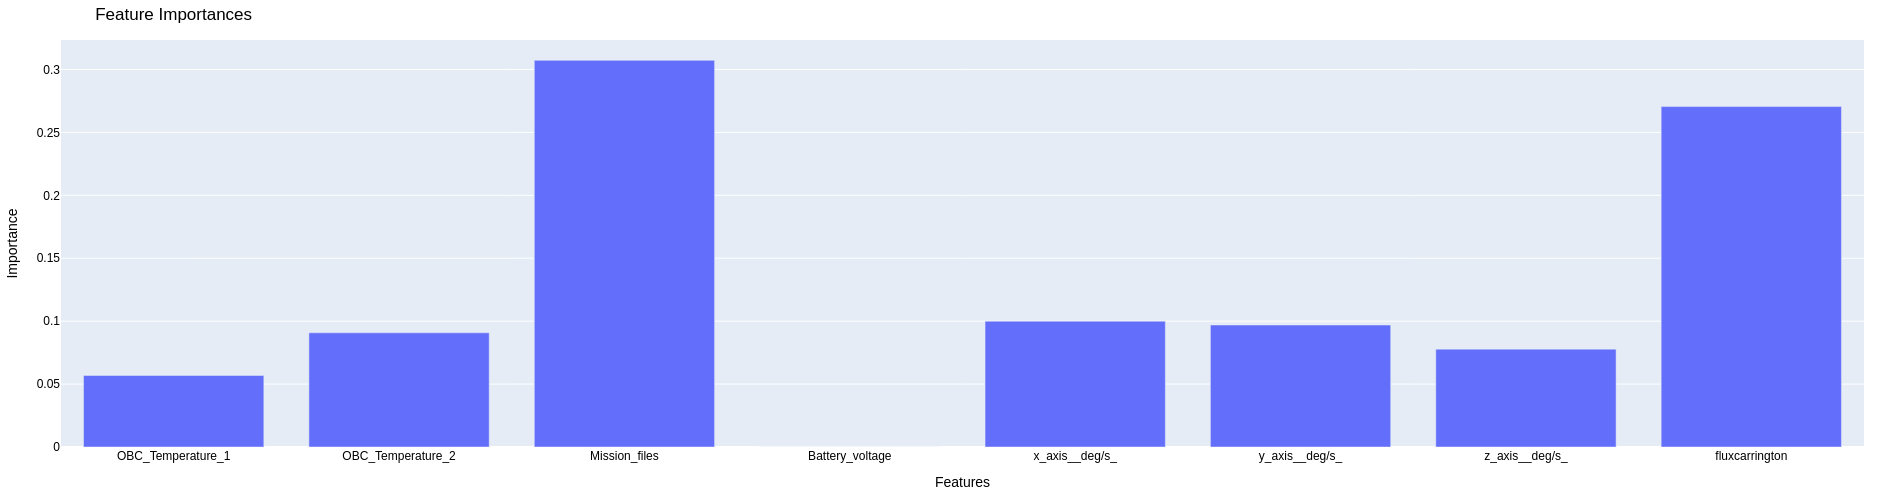
\includegraphics[width=1.0\textwidth]{feature_importances_example.png}
	\caption{Важность признаков в модели XGBoost}
	\label{fig:feature_importances} \end{figure}

\subsection{Сравнение Экспериментов}

Одной из наиболее ценных возможностей MLflow является сравнение
различных экспериментов с разными гиперпараметрами. На графике
\ref{fig:mlflow_comparison} показано сравнение результатов
нескольких экспериментов, включая метрики, такие как точность
(accuracy) и ошибка предсказания (loss), в зависимости от выбранных
гиперпараметров. Это позволяет пользователю выбрать наиболее
оптимальную модель для дальнейшего использования.

\begin{figure}[h!] \centering
	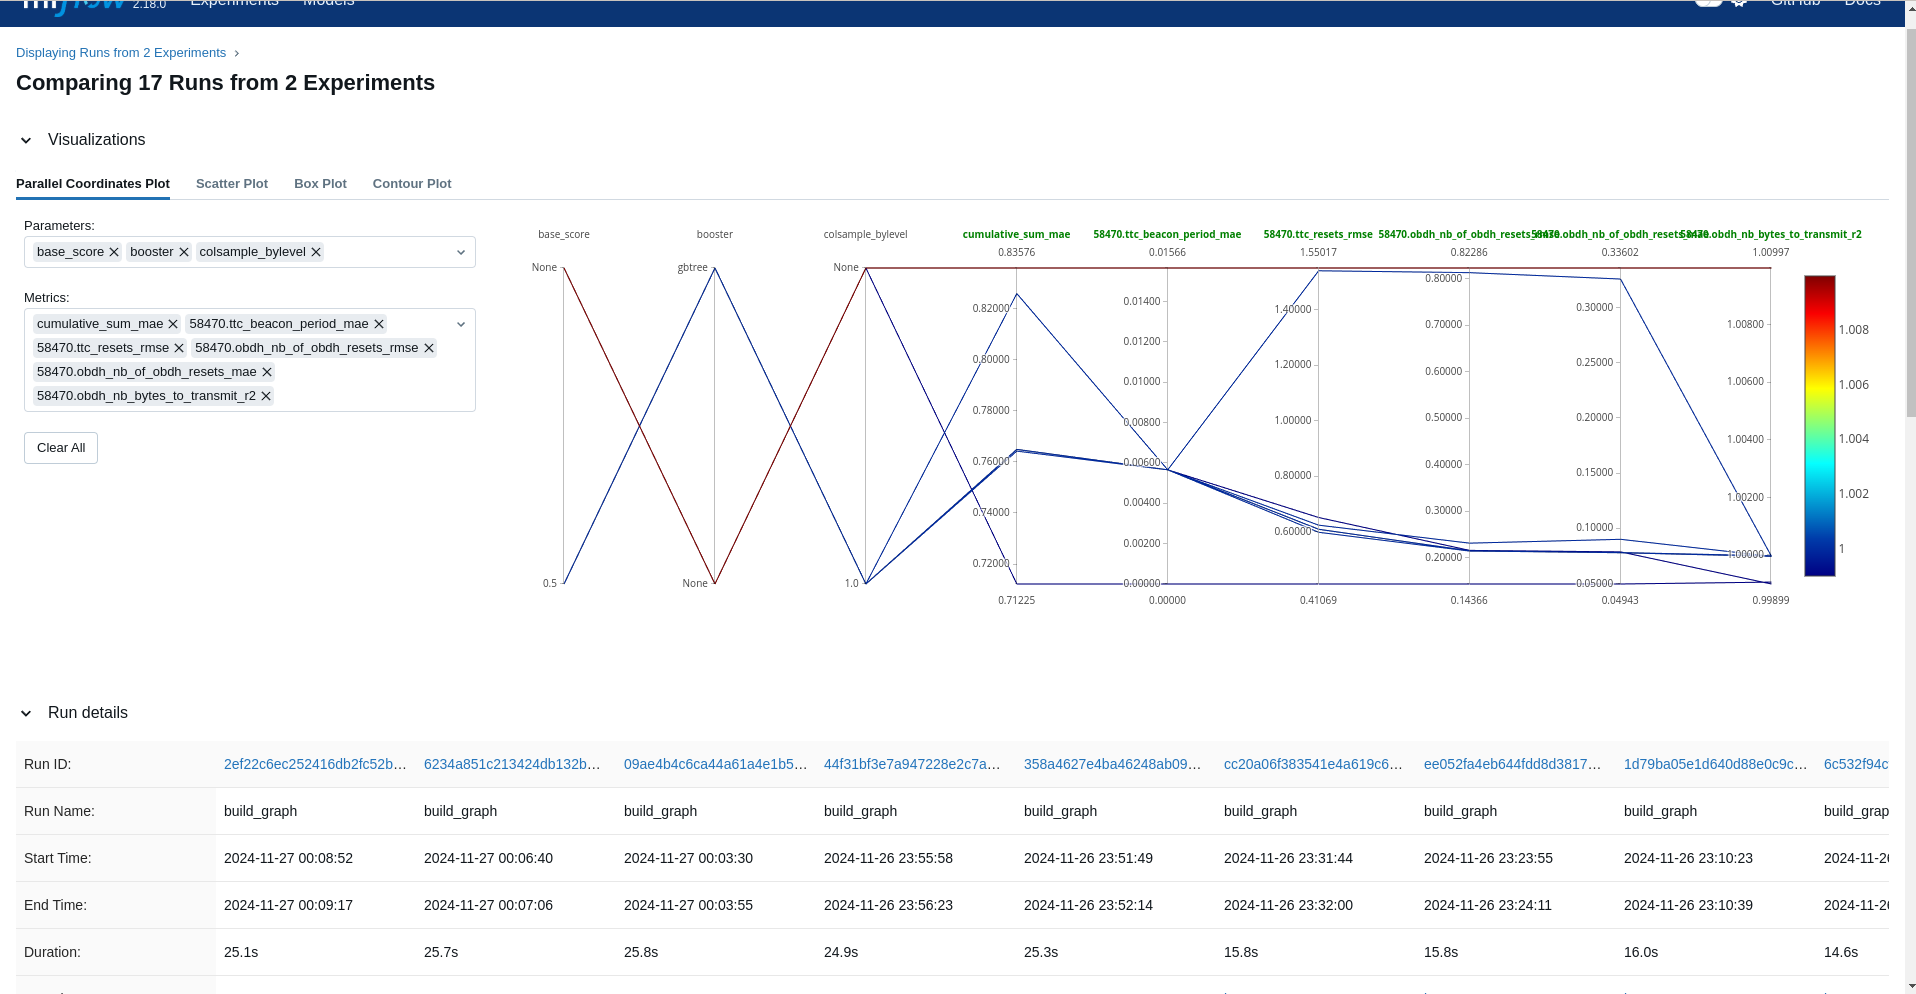
\includegraphics[width=1.0\textwidth]{mlflow_comparision_of_experiments.png}
	\caption{Сравнение различных экспериментов в MLflow}
	\label{fig:mlflow_comparison} \end{figure}

\subsection{Системные Метрики}

MLflow также отслеживает системные метрики, такие как использование
процессора, памяти и GPU, что критически важно при обучении больших
моделей. Эти метрики помогают понять, насколько эффективно
используются вычислительные ресурсы, и могут подсказать, где есть
узкие места в процессе обучения. Рисунок
\ref{fig:mlflow_system_metrics} иллюстрирует, как MLflow
отслеживает и визуализирует использование системных ресурсов.

\begin{figure}[h!] \centering
	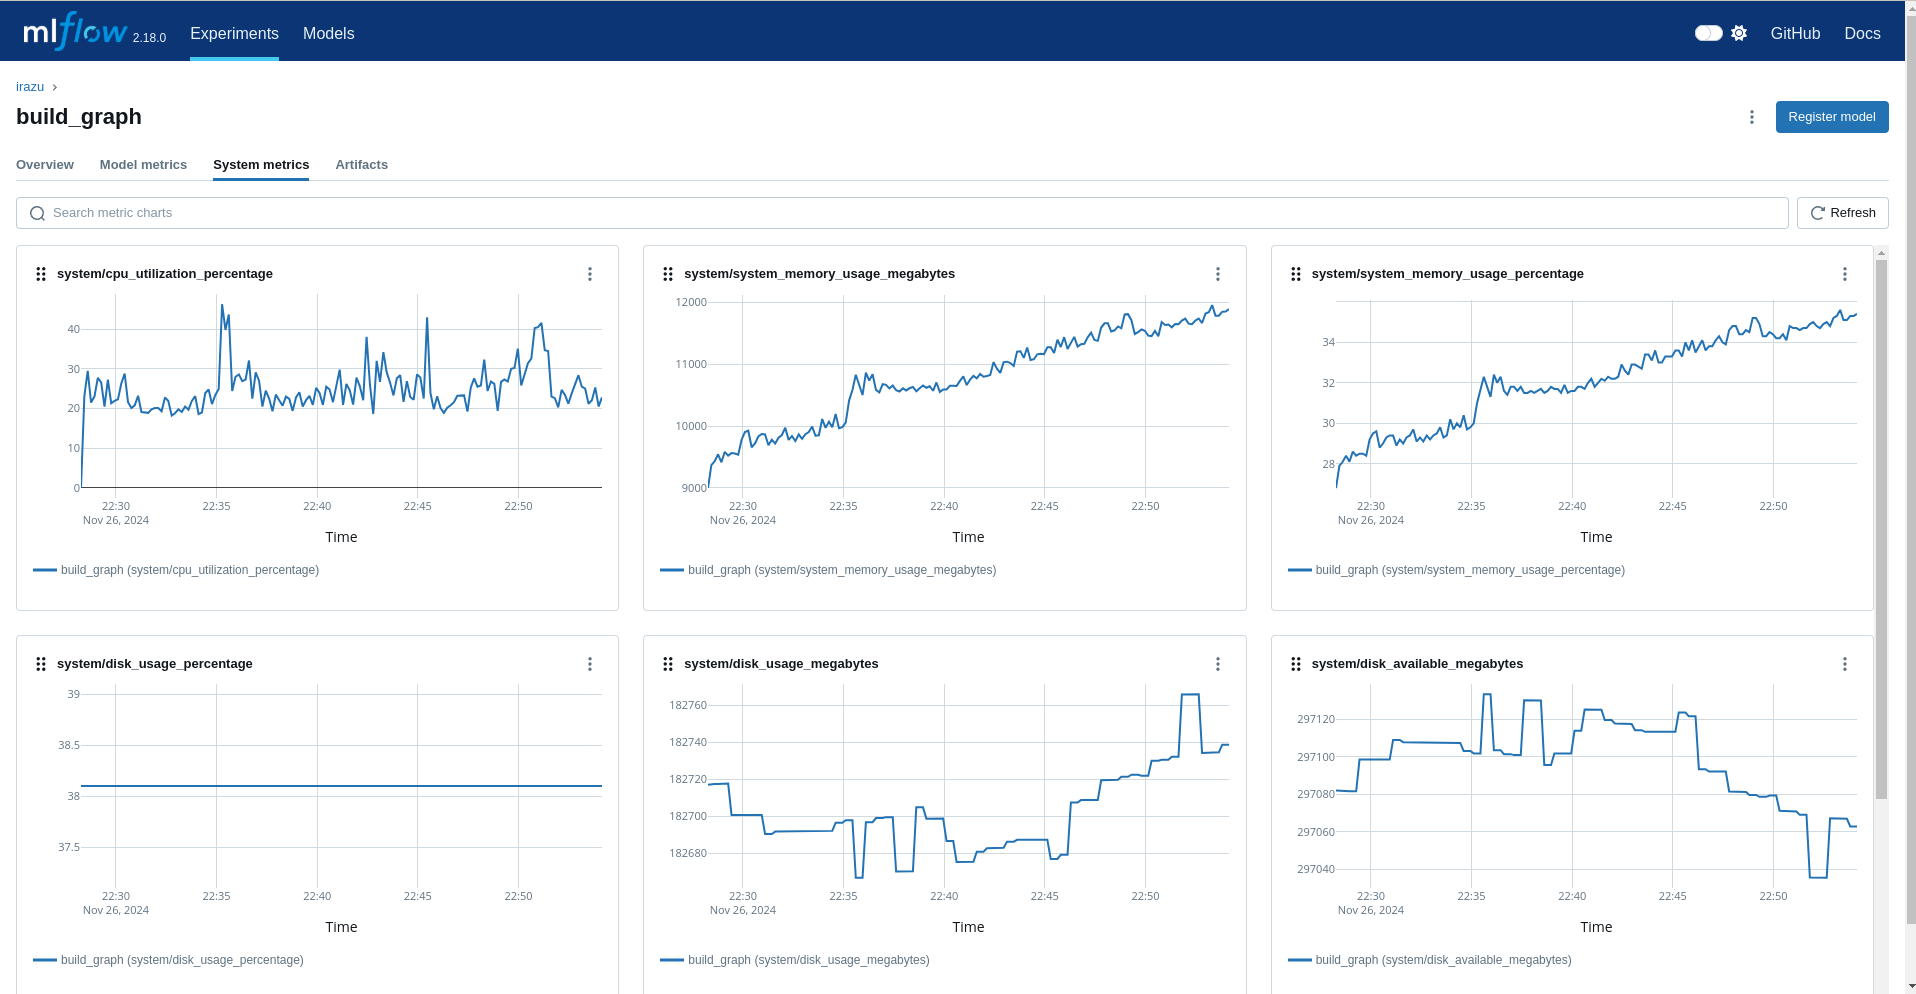
\includegraphics[width=1.0\textwidth]{mlflow_system_metrics_example.png}
	\caption{Системные метрики в MLflow}
	\label{fig:mlflow_system_metrics} \end{figure}

\section{Анализ Результатов Экспериментов}

Одним из важнейших аспектов работы с MLflow является анализ
результатов экспериментов. Для этого используются различные
визуализации и метрики, такие как графики ошибок и предсказаний,
которые наглядно показывают, насколько хорошо модель выполняет свою
задачу.

\subsection{Предсказания против Реальных Значений}

График \ref{fig:prediction_vs_actual} показывает сравнение
предсказанных значений с реальными значениями. Это важно для оценки
точности модели. Чем меньше расхождения между предсказаниями и
реальными значениями, тем выше качество модели.

\begin{figure}[h!] \centering
	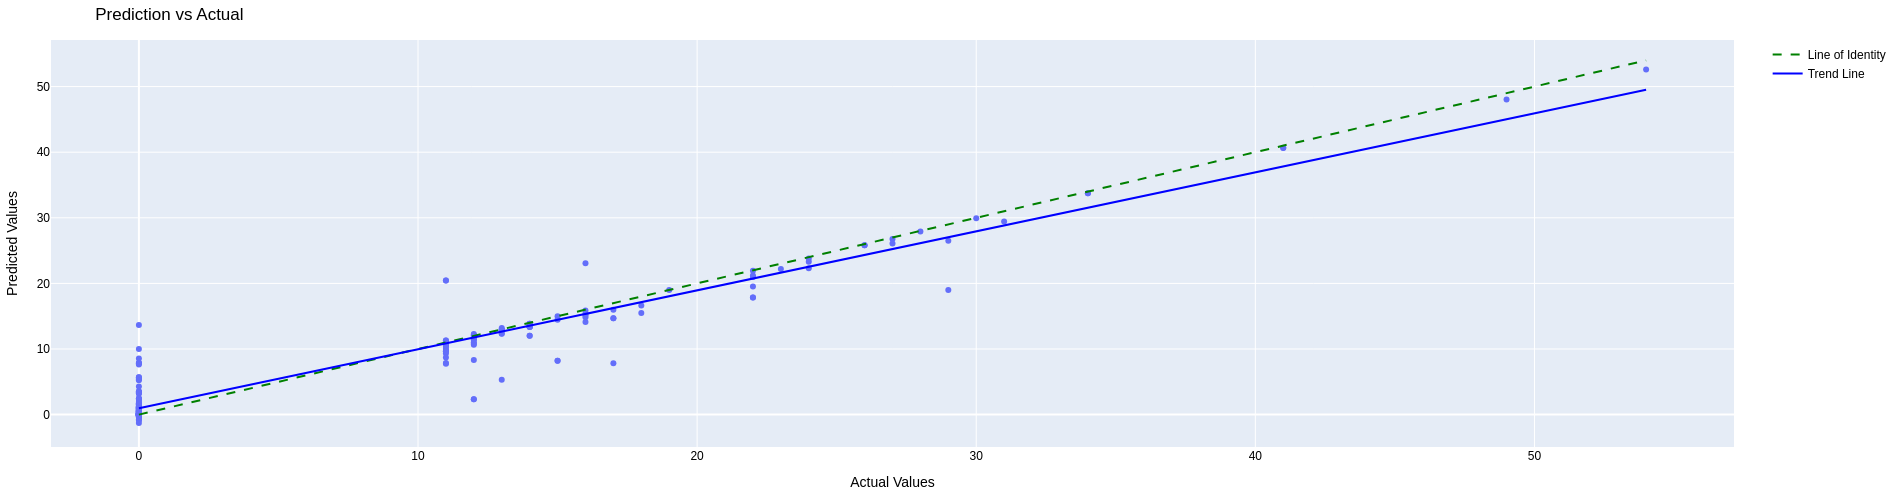
\includegraphics[width=1.0\textwidth]{prediction_vs_actual_example.png}
	\caption{Сравнение предсказаний и реальных значений}
	\label{fig:prediction_vs_actual} \end{figure}

\subsection{Остатки Предсказания}

Для оценки точности и стабильности модели также анализируются
остатки предсказания, которые показывают разницу между
предсказанными и фактическими значениями. График на рисунке
\ref{fig:residuals} демонстрирует распределение остатков модели,
что позволяет понять, как хорошо модель предсказывает данные и где
возникают наибольшие ошибки.

\begin{figure}[h!] \centering
	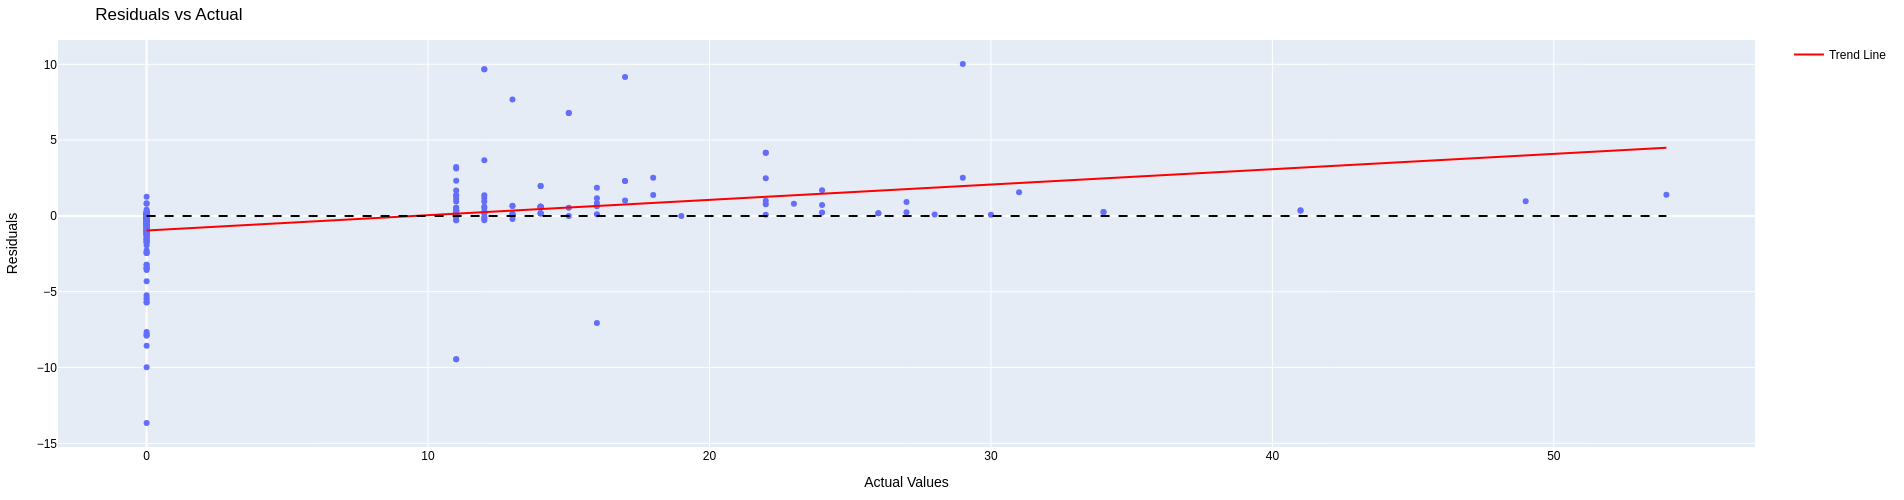
\includegraphics[width=1.0\textwidth]{residuals_example.png}
	\caption{Остатки предсказаний модели} \label{fig:residuals}
\end{figure}

\subsection{Распределение Остаточных Ошибок}

Для более детального анализа ошибок модели используется
распределение остатков. На рисунке \ref{fig:residuals_distribution}
показано, как распределяются ошибки модели на различных этапах ее
обучения. Это помогает выявить возможные проблемы, такие как
смещение модели или избыточная вариативность, которая может быть
устранена через дополнительные корректировки.

\begin{figure}[h!] \centering
	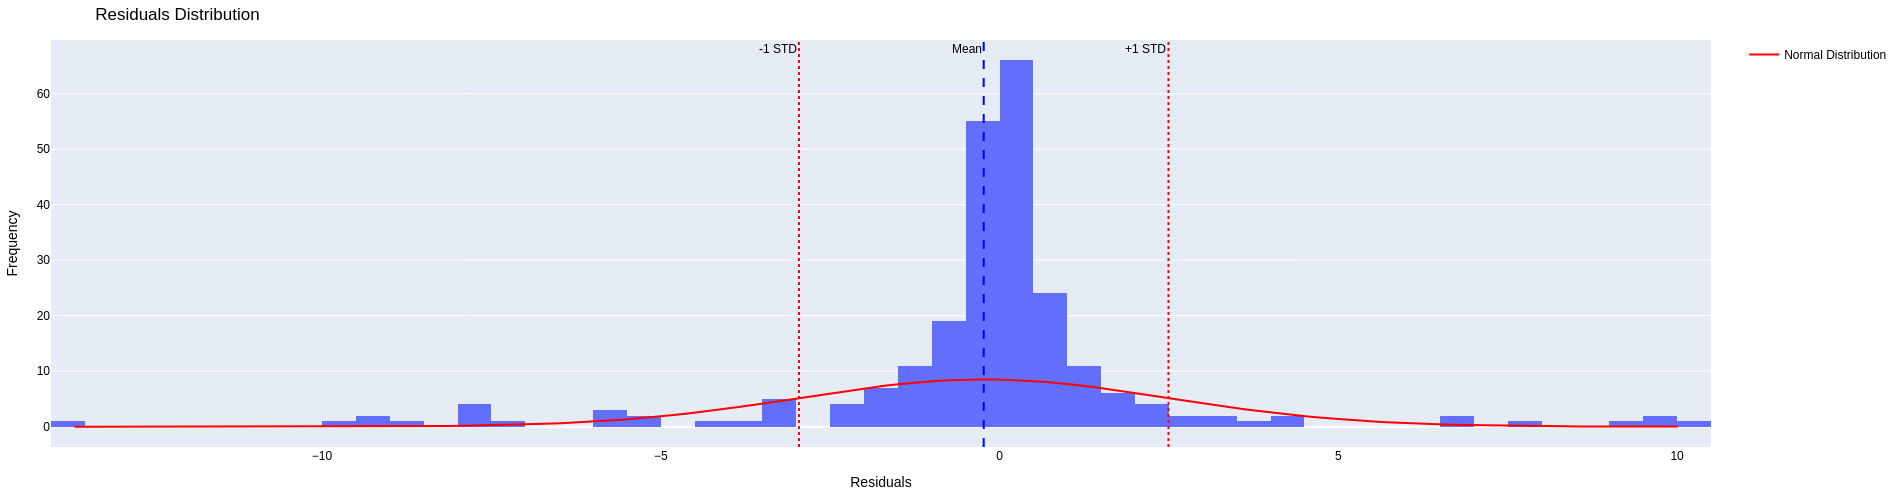
\includegraphics[width=1.0\textwidth]{residuals_distribution_example.png}
	\caption{Распределение остаточных ошибок}
	\label{fig:residuals_distribution} \end{figure}

\subsection{Артефакты MLflow}

После завершения экспериментов все полученные артефакты, такие как
модели, метрики и визуализации, сохраняются в систему и могут быть
использованы для дальнейшего анализа или воспроизведения
эксперимента. Например, на рисунке \ref{fig:mlflow_artifacts}
показан пример артефактов, которые были сохранены в процессе одного
из экспериментов.

\begin{figure}[h!] \centering
	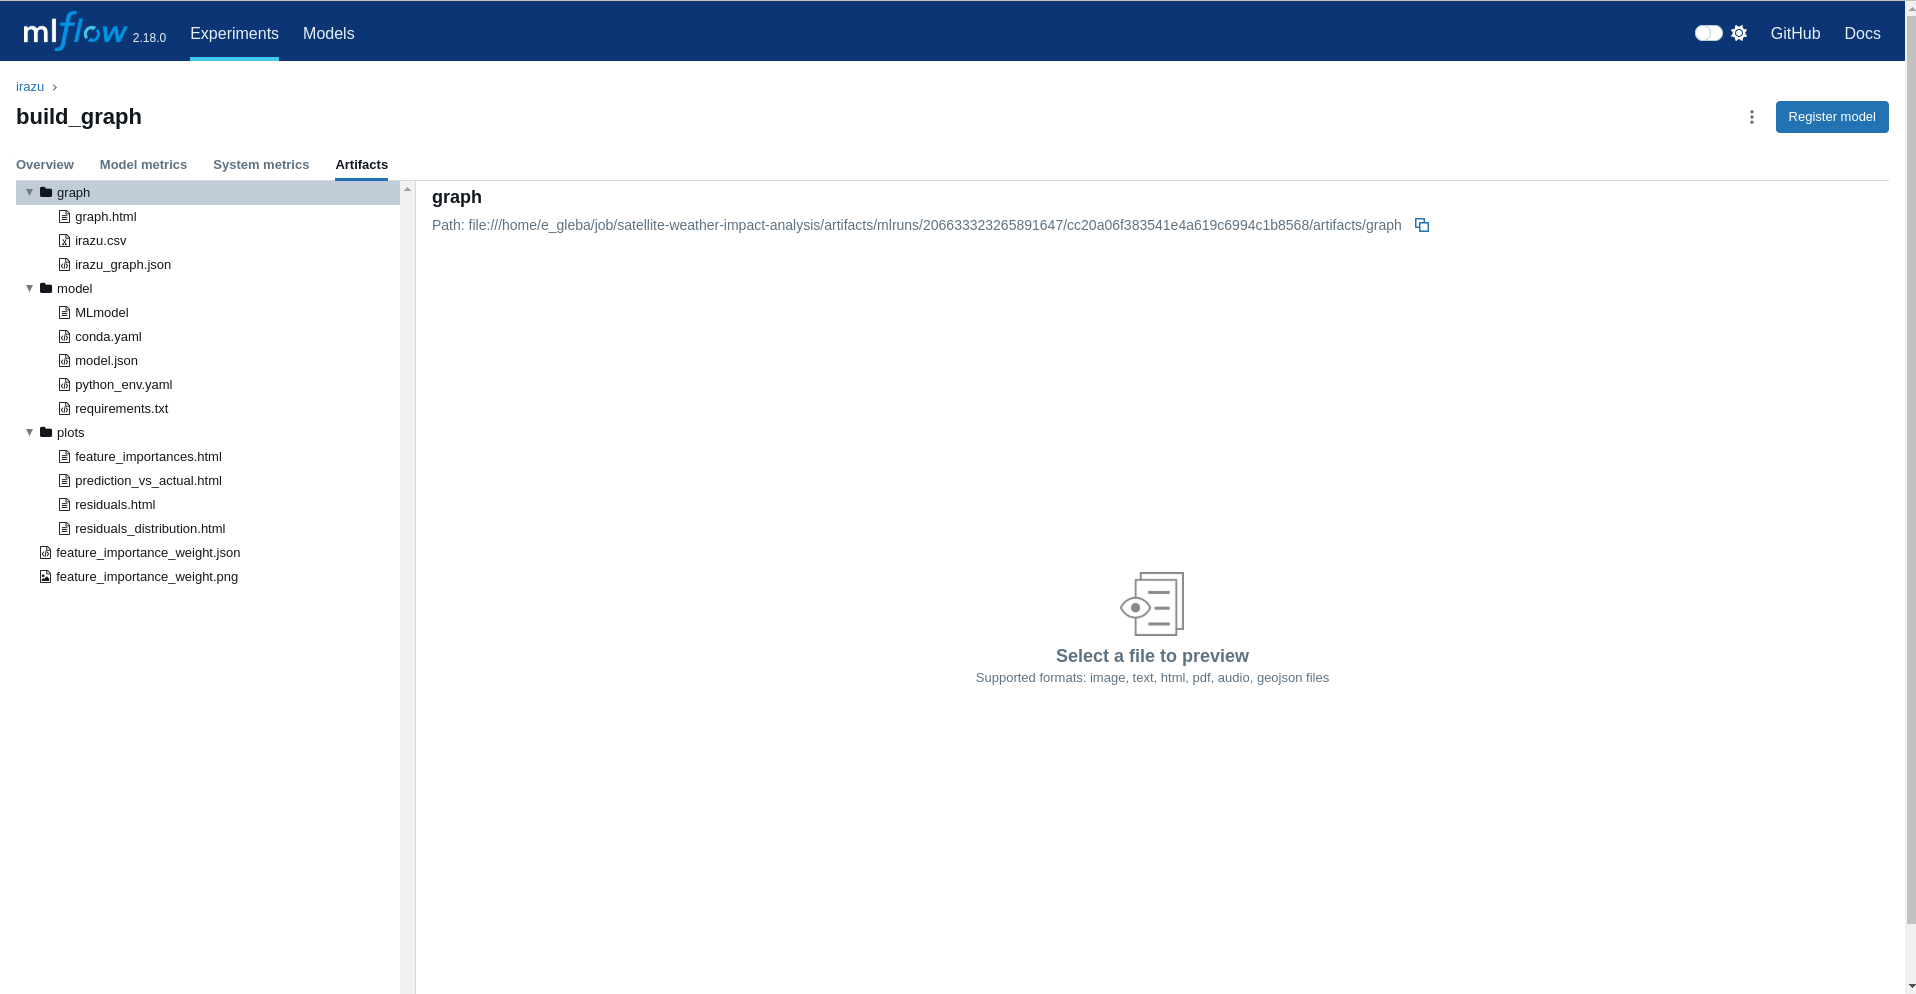
\includegraphics[width=1.0\textwidth]{mlflow_artifacts_example.png}
	\caption{Артефакты эксперимента в MLflow}
	\label{fig:mlflow_artifacts} \end{figure}

\section{Заключение}

Интеграция MLflow в платформу Polaris ML существенно повысила
возможности для отслеживания и анализа экспериментов. MLflow не
только помогает автоматизировать процесс ведения отчетности, но и
позволяет эффективно сравнивать результаты, анализировать метрики и
артефакты, что способствует оптимизации моделей и улучшению
качества прогнозирования. В дальнейшем планируется расширение
функционала MLflow, включая интеграцию с дополнительными типами
артефактов и метрик, что позволит еще больше улучшить процессы
MLOps и повысить производительность системы.

\newpage

\chapter{Анализ графов спутников полученных при помощи polaris 2.0}

Для оценки влияния космической погоды на бортовые системы и целевую
аппаратуру малых космических аппаратов (МКА) будет проведен
комплексный анализ зависимости параметров телеметрии
\cite{green_2017_impact} \cite{schlag_2018_numerical}
\cite{boumghar_2018_enhanced}, индексов солнечной активности и
геомагнитных индексов. В основе исследования лежит применение
модели машинного обучения Polaris ML. Результаты работы модели
будут представлены в виде двухмерного графа связности, отражающего
выявленные взаимосвязи между исследуемыми параметрами.

Для расчета и анализа графа связности будет использована обширная
база данных телеметрии сети наземных станций SatNOGS. Параметры
солнечной активности будут извлечены из следующих источников:

\begin{itemize} \item Центр прогнозирования космической погоды (Space
	      Weather Prediction Center, SWPC/SWO) \cite{swpc_noaa_data_souce};
	\item Центр наблюдения и анализа данных о влиянии Солнца в Брюсселе
	      (Solar Influences Data Analysis Center, S.I.D.C.)
	      \cite{silso_snd_data_source}; \item Канадская
	      радиоастрофизическая обсерватория в Пентиктоне
	      \cite{swgc_flux_data_source}. \end{itemize}

Процесс исследования состоит из нескольких этапов:

\paragraph*{1. Извлечение и обработка данных.} На первом этапе
выполняется автоматическое извлечение данных телеметрии из базы сети
наземных станций SatNOGS за весь период функционирования целевого
спутника или за выбранный временной интервал. Параллельно
производится сбор параметров солнечной активности из баз данных SWPC,
S.I.D.C. и канадской радиоастрофизической обсерватории в Пентиктоне.

\paragraph*{2. Применение методов машинного обучения.} На втором
этапе используется алгоритм XGBoost для анализа взаимосвязей между
собранными данными. В результате работы модели формируется JSON-файл,
содержащий ключевые параметры графа связности.

\paragraph*{3. Построение графа связности и анализ результатов.}
Заключительный этап включает визуализацию результатов в виде 2D-графа
связности. Этот граф позволяет исследовать взаимодействие между
параметрами, выявить ключевые факторы, влияющие на работу бортовых
систем, и оценить степень их чувствительности к космической погоде.

\begin{longtable}{|l|p{12cm}|} \caption{Подробное описание параметров
		солнечной и геомагнитной активности}
	\label{tab:detailed_solar_geo_params}
	\\

	\hline \textbf{Параметр} & \textbf{Описание}
	\\ \hline \endfirsthead

	\multicolumn{2}{c}% {\tablename\ \thetable\ --
	\textit{Продолжение}}
	\\ \hline \textbf{Параметр}     & \textbf{Описание}
	\\ \hline \endhead

	\hline \multicolumn{2}{|r|}{\textit{Продолжение на следующей
			странице}}
	\\ \hline \endfoot

	\hline \endlastfoot

	ssn                      & Среднемесячное число солнечных пятен —
	ключевой индикатор солнечной активности, получаемый Центром
	наблюдения и анализа данных о влиянии Солнца в Брюселе (S.I.D.C.).
	Солнечные пятна представляют собой области с пониженной
	температурой, вызванные магнитными полями, которые препятствуют
	конвективным процессам. Их количество варьируется в зависимости от
	11-летнего цикла солнечной активности, что делает ssn важным
	параметром для понимания солнечного поведения и его влияния на
	космическую погоду.                                               \\ \hline smoothed\_ssn         & Сглаженное
	число солнечных пятен — это усредненное значение количества
	солнечных пятен за определенный период, также предоставляемое
	S.I.D.C. Сглаживание позволяет устранить краткосрочные колебания и
	выявить долгосрочные тенденции в солнечной активности, что
	критически важно для прогноза космической погоды и оценки
	воздействия на Землю.
	\\ \hline observed\_swpc\_ssn   & Среднемесячное число солнечных
	пятен, зарегистрированное Центром прогнозирования космической
	погоды (SWPC/SWO). Этот параметр служит основой для оценки текущего
	состояния солнечной активности и ее потенциального влияния на
	магнитосферу Земли, что имеет значение для защиты спутников и
	других технологий.
	\\ \hline smoothed\_swpc\_ssn   & Сглаженное число солнечных пятен,
	полученное из наблюдений SWPC/SWO. Оно позволяет анализировать
	долгосрочные изменения в солнечной активности, что особенно полезно
	для научных исследований и разработки моделей предсказания
	космической погоды.
	\\ \hline f10.7                 & Среднемесячные значения потока
	радиоизлучения на длине волны 10,7 см — важный индикатор солнечной
	активности, измеряемый канадской радиоастрофизической обсерваторией
	в Пентиктоне, Британская Колумбия. Этот параметр коррелирует с
	количеством солнечных пятен и служит основным показателем для
	оценки интенсивности радиоволн, излучаемых Солнцем.
	\\ \hline smoothed\_f10.7       & Сглаженные значения потока
	радиоизлучения 10,7 см, которые помогают устранить кратковременные
	колебания и выявить более стабильные тренды в солнечной радиации,
	что имеет критическое значение для исследований климатических
	изменений и космической погоды.
	\\ \hline observed flux         & Наблюдаемое значение солнечного
	излучения — это интегральная мера выбросов энергии от Солнца,
	полученная с помощью радиотелескопов. Это значение подвержено
	модуляции двумя основными факторами: уровнем солнечной активности и
	изменением расстояния между Землей и Солнцем, что делает его важным
	для понимания динамики солнечного излучения и его воздействия на
	земную атмосферу.
	\\ \hline adjusted flux         & Скорректированное наблюдаемое
	значение солнечного излучения, которое учитывает изменения
	расстояния между Землей и Солнцем, предоставляя более точную оценку
	энергии, достигающей нашей планеты. Этот параметр важен для
	климатических исследований и оценки воздействия солнечной
	активности на земную экосистему.
	\\ adjusted flux         & Наблюдаемое значение солнечного
	излучения, скорректированное на изменения расстояния между Землей и
	Солнцем и данное для среднего расстояния.
	\\ \hline Obs-time              & Время наблюдения. Указывает
	точный временной интервал, связанный с измерениями. Обычно
	представлено в формате UTC (Coordinated Universal Time) для
	обеспечения стандартизации данных по всему миру. Формат: YYYY-MM-DD
	HH:MM:SS.
	\\ \hline Fredericksburg A      & Индекс магнитной активности в
	районе Фредериксбурга (США). Используется для мониторинга
	геомагнитных изменений. Представляет собой линейную шкалу,
	отражающую амплитуду возмущений магнитного поля Земли. Единица
	измерения: нанотесла (нТл). Диапазон значений: от 0 до 400 нТл.
	\\ \hline Fredericksburg K 0-3  & Категории магнитной активности
	K-индекса (низкий уровень, 0-3) в Фредериксбурге. K-индекс
	измеряется каждые три часа и отражает локальные геомагнитные
	возмущения. Безразмерная величина. Соответствует возмущениям до 20
	нТл.
	\\ \hline Fredericksburg K 3-6  & Категории магнитной активности
	K-индекса (умеренный уровень, 3-6) в Фредериксбурге. Указывает на
	усиление геомагнитной активности. Безразмерная величина.
	Соответствует возмущениям от 20 до 120 нТл.
	\\ \hline Fredericksburg K 6-9  & Категории магнитной активности
	K-индекса (высокий уровень, 6-9) в Фредериксбурге. Свидетельствует
	о сильных геомагнитных возмущениях. Безразмерная величина.
	Соответствует возмущениям от 120 до 300 нТл и выше.
	\\ \hline fluxdate              & Дата измерения солнечного
	радиоизлучения. Важна для отслеживания долгосрочных изменений
	солнечной активности. Формат: YYYY-MM-DD.
	\\ \hline fluxtime              & Время измерения солнечного
	радиоизлучения. Позволяет анализировать краткосрочные колебания
	солнечной активности. Формат: HH:MM (UTC).
	\\ \hline fluxjulian            & Юлианская дата, используемая для
	астрономических вычислений. Обеспечивает непрерывную шкалу времени,
	удобную для расчетов. Единица измерения: дни. Точность: до 5 знаков
	после запятой.
	\\ \hline fluxcarrington        & Номер периода вращения
	Каррингтона для корреляции солнечного излучения. Используется для
	отслеживания солнечных явлений, связанных с вращением Солнца.
	Безразмерная величина. Период Каррингтона $\approx$ 27.2753 дня.
	\\ \hline fluxobsflux           & Наблюдаемый поток радиоизлучения
	(10.7 см) на момент измерения. Измеряется в солнечных единицах
	потока (с.е.п., 1 с.е.п. = \(10^{-22}\) Вт·м\(^{-2}\)·Гц\(^{-1}\)).
	Является важным индикатором солнечной активности.
	\\ \hline fluxadjflux           & Приведенный поток радиоизлучения
	(с поправкой на расстояние между Землей и Солнцем). Позволяет
	сравнивать данные, полученные в разные периоды года. Единица
	измерения: с.е.п.
	\\ \hline fluxursi              & Поток URSI, принятый стандарт в
	радиофизике для солнечного радиоизлучения. Обеспечивает
	стандартизированное измерение солнечного радиопотока. Единица
	измерения: с.е.п.
	\\ \hline SNvalue (hemispheric) & Наблюдаемое число солнечных пятен
	по полушариям. Важный показатель солнечной активности, отражающий
	асимметрию активности Солнца. Безразмерная величина.
	\\ \hline SNerror (hemispheric) & Ошибка в оценке числа солнечных
	пятен по полушариям. Указывает на точность измерений и возможные
	погрешности. Безразмерная величина.
	\\ \hline Nb\_observations      & Количество наблюдений,
	использованных для вычисления параметров. Важно для оценки
	статистической значимости данных. Целое число.
	\\\end{longtable}

Для выявления взаимосвязей между параметрами солнечной активности и
параметрами бортовой электроники и полезной нагрузки использовались
данные телеметрии для следующих спутников: CSIM-FD (NORAD: 43793),
CTIM (NORAD: 52950), ENSO (NORAD: 58470), GRBAlpha (NORAD: 47959),
GREENCUBE (NORAD: 53106).


\newpage

% Conclusion (centered section format)
\titleformat{\section}[block]{\large\bfseries\filcenter}{}{0em}{}
\nonPrefixChapter{Заключение}

\newpage

% Bibliography
\printbibliography[heading=bibintoc,title={Список использованной литературы}]

\newpage

% Appendices
\appendix

\renewcommand{\chaptermark}[1]{\markboth{}{}}
\renewcommand{\sectionmark}[1]{\markright{\arabic{section}.\ #1}}

% Fix for malformed section formatting
\titleformat{\section}[block]{\large\bfseries\filcenter}{}{0em}{}

\nonPrefixChapter{Приложения} \label{sec:attachements}

\section{Приложение \arabic{section}}
\label{subsec:old_polaris_learn_config}

В данном приложении представлена старая конфигурация, используемая для формирования нейронного ансамбля с помощью алгоритма XGBoost.

\lstinputlisting[language=Java, label={lst:old_polaris_config}, caption=Конфигурация XGBoost]{../code/old_polaris_cfg.json}

\end{document}
